\section{Shape Sensitivity Analysis for 1D problem}
% ================================================
For the first benchmark case, we looked at the flow between two plates that was defined in Section \ref{sec:C3_benchmark_case}. The governing equation and boundary conditions for this problem is shown in Equation \eqref{eq:C4_1DbenchmarkProblem}. The boundary condition is defined as $u = U$ at $y = L$.

\begin{subequations}\label{eq:C4_1DbenchmarkProblem}
\begin{equation}\label{eq:C4_1DbenchmarkGoverningEquation}
    u_t = \mu u_{yy} \quad \text{in } \Omega_f
\end{equation}
\begin{equation}\label{eq:C4_1DbenchmarkBoundaryCondition}
\begin{cases}
    u = U \quad \text{at } y = 0 \\
    u = 0 \quad \text{at } y = L
\end{cases}
\end{equation}
\end{subequations}

The analytical result for the steady-state velocity profile between the two plates is defined in Equation \eqref{eq:C4_1DbenchmarkAnalyticalSolution}

\begin{equation}\label{eq:C4_1DbenchmarkAnalyticalSolution}
	u = U\frac{L - x}{L}
\end{equation}

This enables us to treat the moving wall velocity ($U$) and the distance between the two plates ($L$) as design variables. The sensitivity of steady-state velocity profile between the two plate to these design variables are calculated using CSA. The results of the CSA are verified with the analytical sensitivity results in Equation \eqref{eq:C4_1DbenchmarkAnalyticalSensitivityResults}.

\begin{subequations}\label{eq:C4_1DbenchmarkAnalyticalSensitivityResults}
\begin{equation}\label{eq:C4_1DbenchmarkAnalyticalSAlength}
	\frac{\partial u}{\partial L} = \frac{Ux}{L^2}
\end{equation}
\begin{equation}\label{eq:C4_1DbenchmarkAnalyticalSAvelocity}
	\frac{\partial u}{\partial U} = \frac{L - x}{L}
\end{equation}
\end{subequations}

For this benchmark problem, the flow is modeled using two different immersed boundary techniques introduced in the beginning of this chapter, penalization method and the virtual boundary method. This difference between the analysis of flow from Chapter \ref{ch:immersedBoundary} is the use of RH and RD functions instead of discontinuous step and delta function. Therefore, first the effect of these modifications are investigated on the simulation results.

For the flow simulation using the penalization method of Equation \eqref{eq:C4_NSwithPenalization} we investigated effect of node number and the moving wall velocity of the accuracy of the solution. To have a stable solution, the time step of flow analysis cannot be bigger that $2 / \kappa$ where $\kappa$ is the porosity value that is selected to model the solid domain. For this analysis the $\eta$ value of the RH function is selected based on the criteria that 99 percent change of the RH function occurs within two mesh cell. The result for the simulation based on RH function is compared with the step function in Figure \ref{fig:C4_effectOfRHfunctionOnSimulationResults1Dproblem}.

\begin{figure}[H]
	\centering
	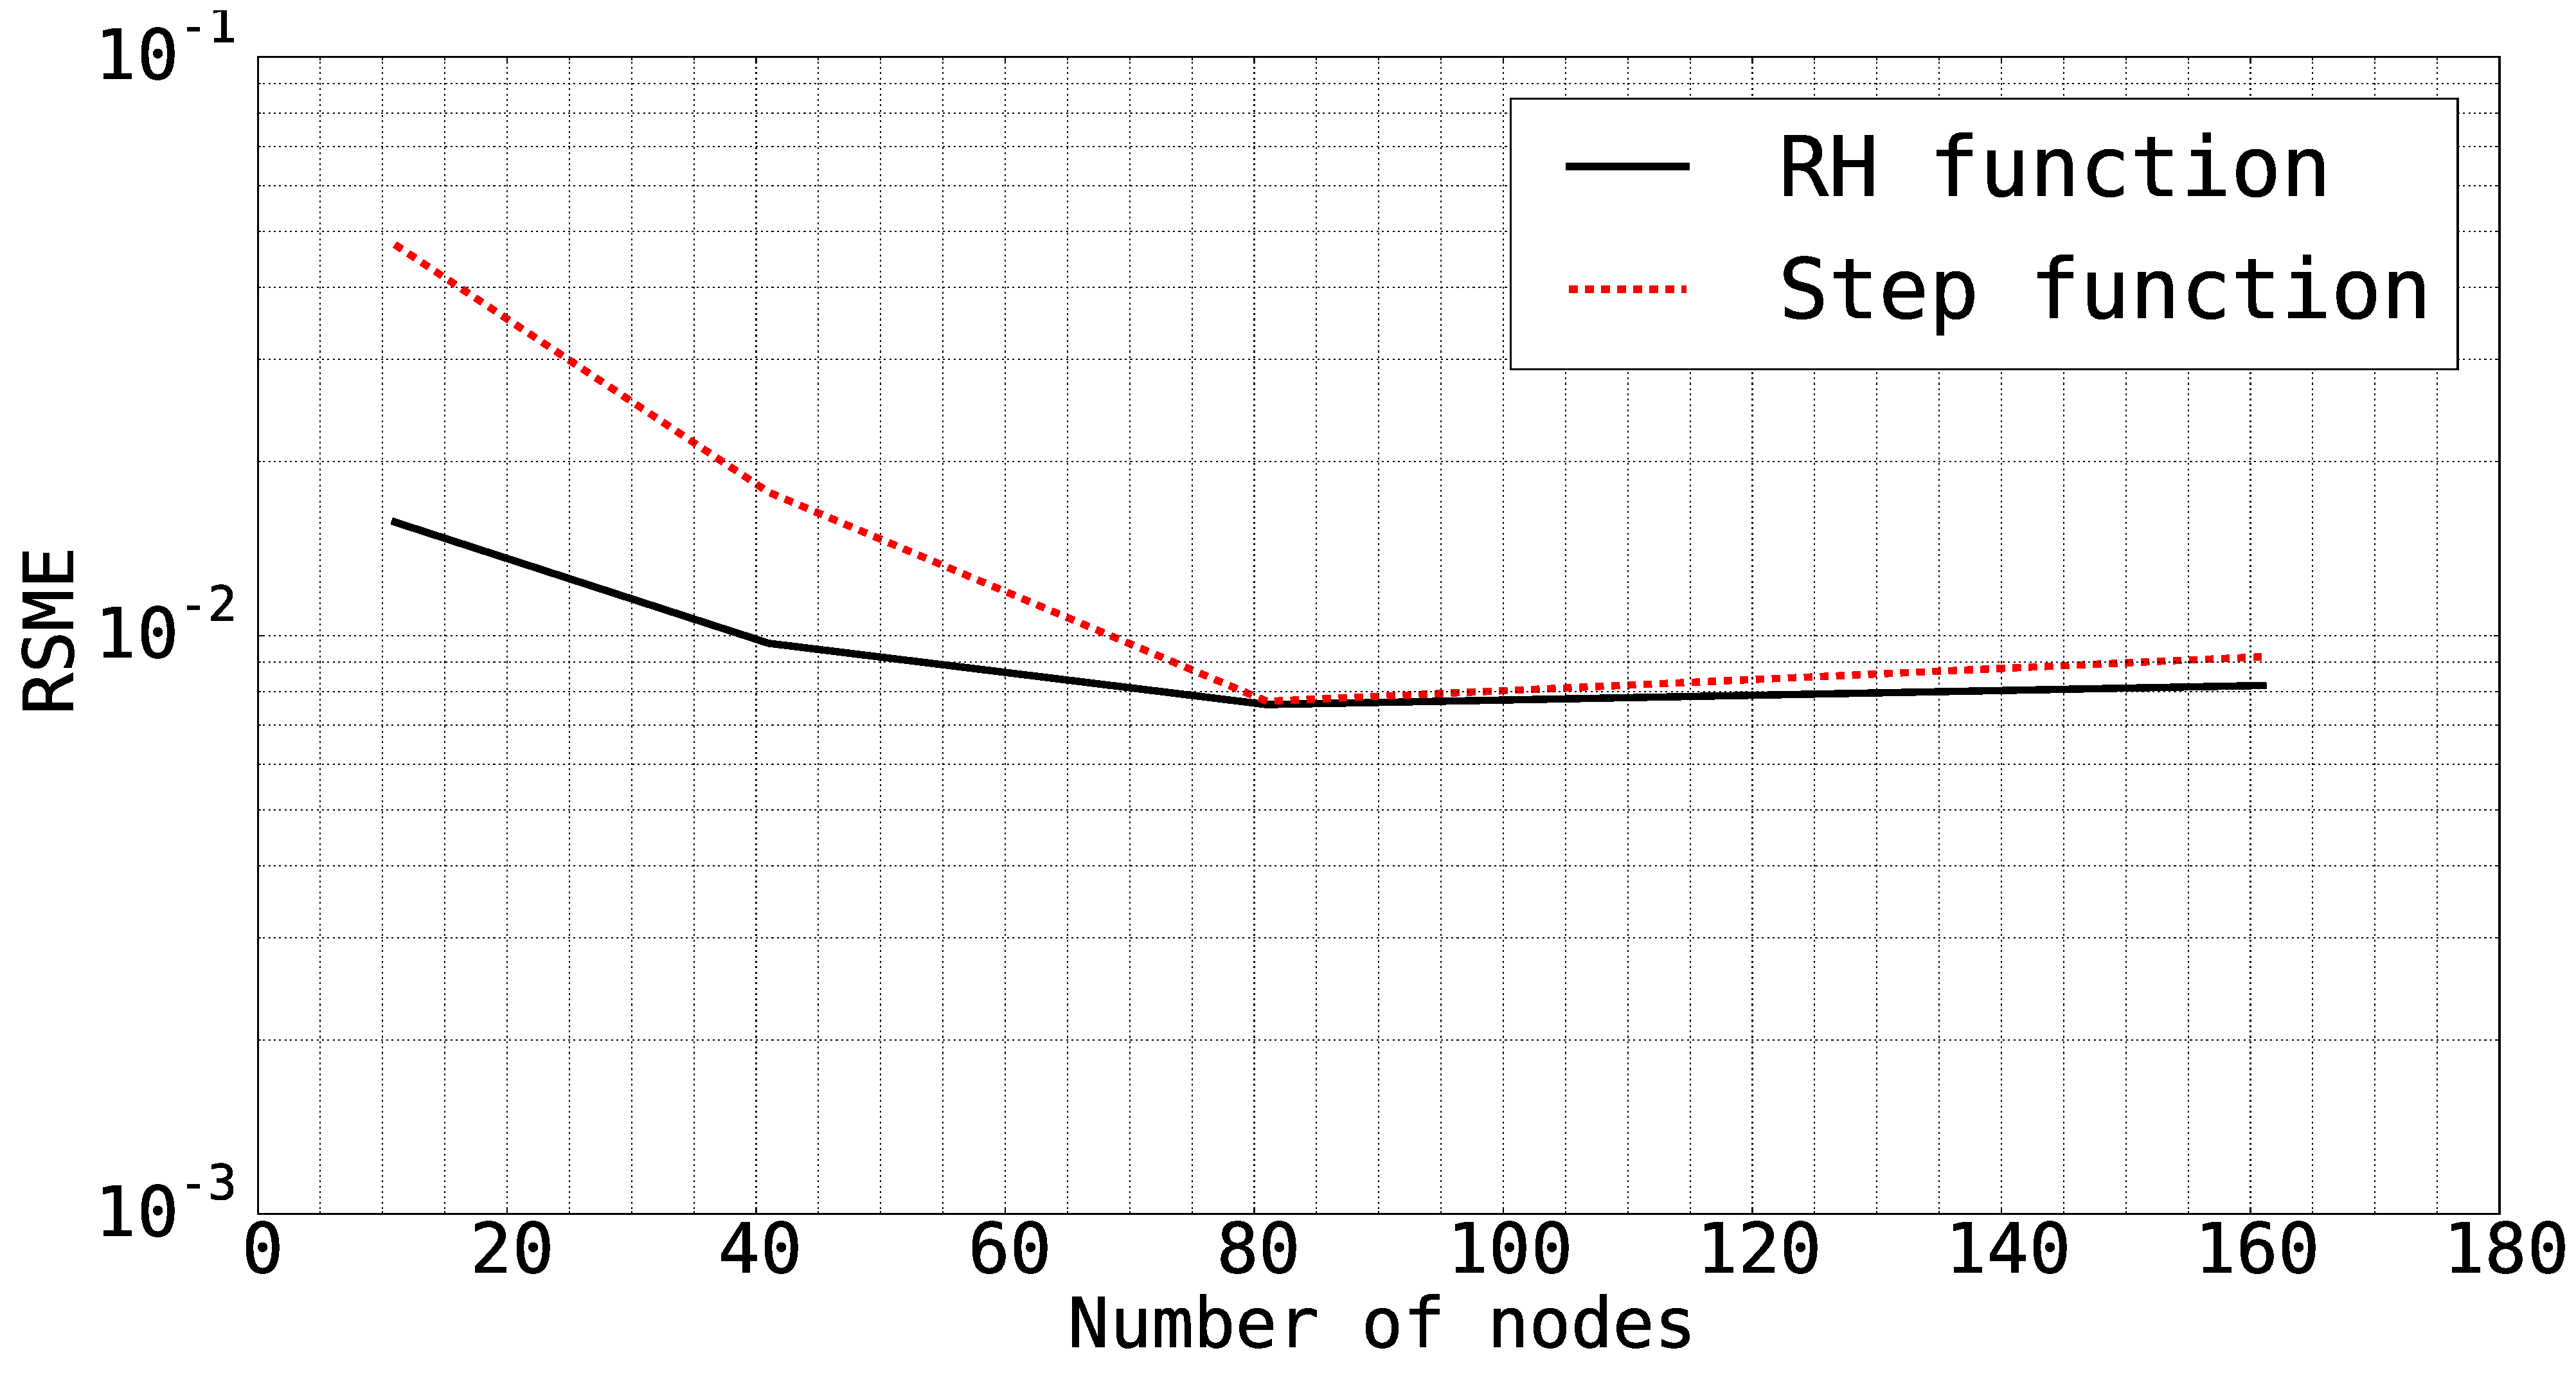
\includegraphics[width=12.00cm]{Chapter_4/figure/effect_of_RH_on_simulation_vs_numberOfNodes_1D_problem.eps}
	\caption{Effect of Regularized Heaviside (RH) and step function on the solution accuracy.}
	\label{fig:C4_effectOfRHfunctionOnSimulationResults1Dproblem}
\end{figure}

As shown in Figure \ref{fig:C4_effectOfRHfunctionOnSimulationResults1Dproblem}, the result of the RH function are more accurate compared to the step function. The effect of wall velocity of the accuracy of the simulation was also investigated. The wall velocity was selected as $1 m/s$, $10 m/s$, $100 m/s$, and $1000 m/s$. However, this did not affect the accuracy of the simulation.

The sensitivity equations for the penalization technique are derived by differentiating the governing equation as shown in Equation \eqref{eq:C4_NSwithPenalizationIBsensitivity}. However, for this problem the convective terms and pressure gradient drop out resulting in the sensitivity equation as shown in Equation \eqref{eq:C4_SAforPenlizationMethod1D}.

\begin{equation}\label{eq:C4_SAforPenlizationMethod1D}
	\frac{\partial u'}{\partial t} = 
	\mu \frac{\partial^2 u'}{\partial x^2} +
	\kappa \left[
	\frac{\partial \mathcal{H}}{\partial X} \frac{\partial X}{\partial b} + 
	\mathcal{H}(X) u'
	\right]
\end{equation}

where $X$ is $x - x_w$ and $x_w$ is the location of the solid wall. $u$ is the flow velocity, $\mu$ is the viscosity, $\kappa$ is the porosity, and $\mathcal{H}$ is the RH function. $b$ corresponds to the generic design variable and $u'$ is the sensitivity of the flow field to the design variable $b$. The boundary conditions are derived by differentiating the Equation \eqref{eq:C4_1DbenchmarkBoundaryCondition}. This is shown in Equation \eqref{eq:C4_SAboundaryConditionforPenlizationMethod1D}. Both of the boundary conditions are zero because their location does not change by changing the design variable.

\begin{equation}\label{eq:C4_SAboundaryConditionforPenlizationMethod1D}
\begin{cases}
	u' = 0 \qquad \text{at } x = 0 \\
	u' = 0 \quad \text{at } x = 1
\end{cases}
\end{equation}

For this problem, the $\kappa$ is selected as $2 \time 10^4$ based on the convergence studies for the governing equations and the sensitivity of the velocity profile with respect to the distance between two plates is verified with Equation \eqref{eq:C4_1DbenchmarkAnalyticalSAlength}. The $\eta$ parameter for the RH function is selected in such a way that 95 percent of change in RH function occurs within two nodes from the solid boundary. This ensures the stability of the method. The initial location of wall is selected as $x_{wall} = 0.4321$ and $x_{wall} = 0.7583$. Neither of these locations coincide with the computational nodes in the domain. The effect of number of nodes on the accuracy of the solution of the governign equations and the sensitivity results are shown in Figure \ref{fig:C4_effectOfNumberOfNodesOnSensitivityResults1Dproblem}.

\begin{figure}[H]
    \centering
    \subfigure[$x_{wall} = 0.4321$]
    {
    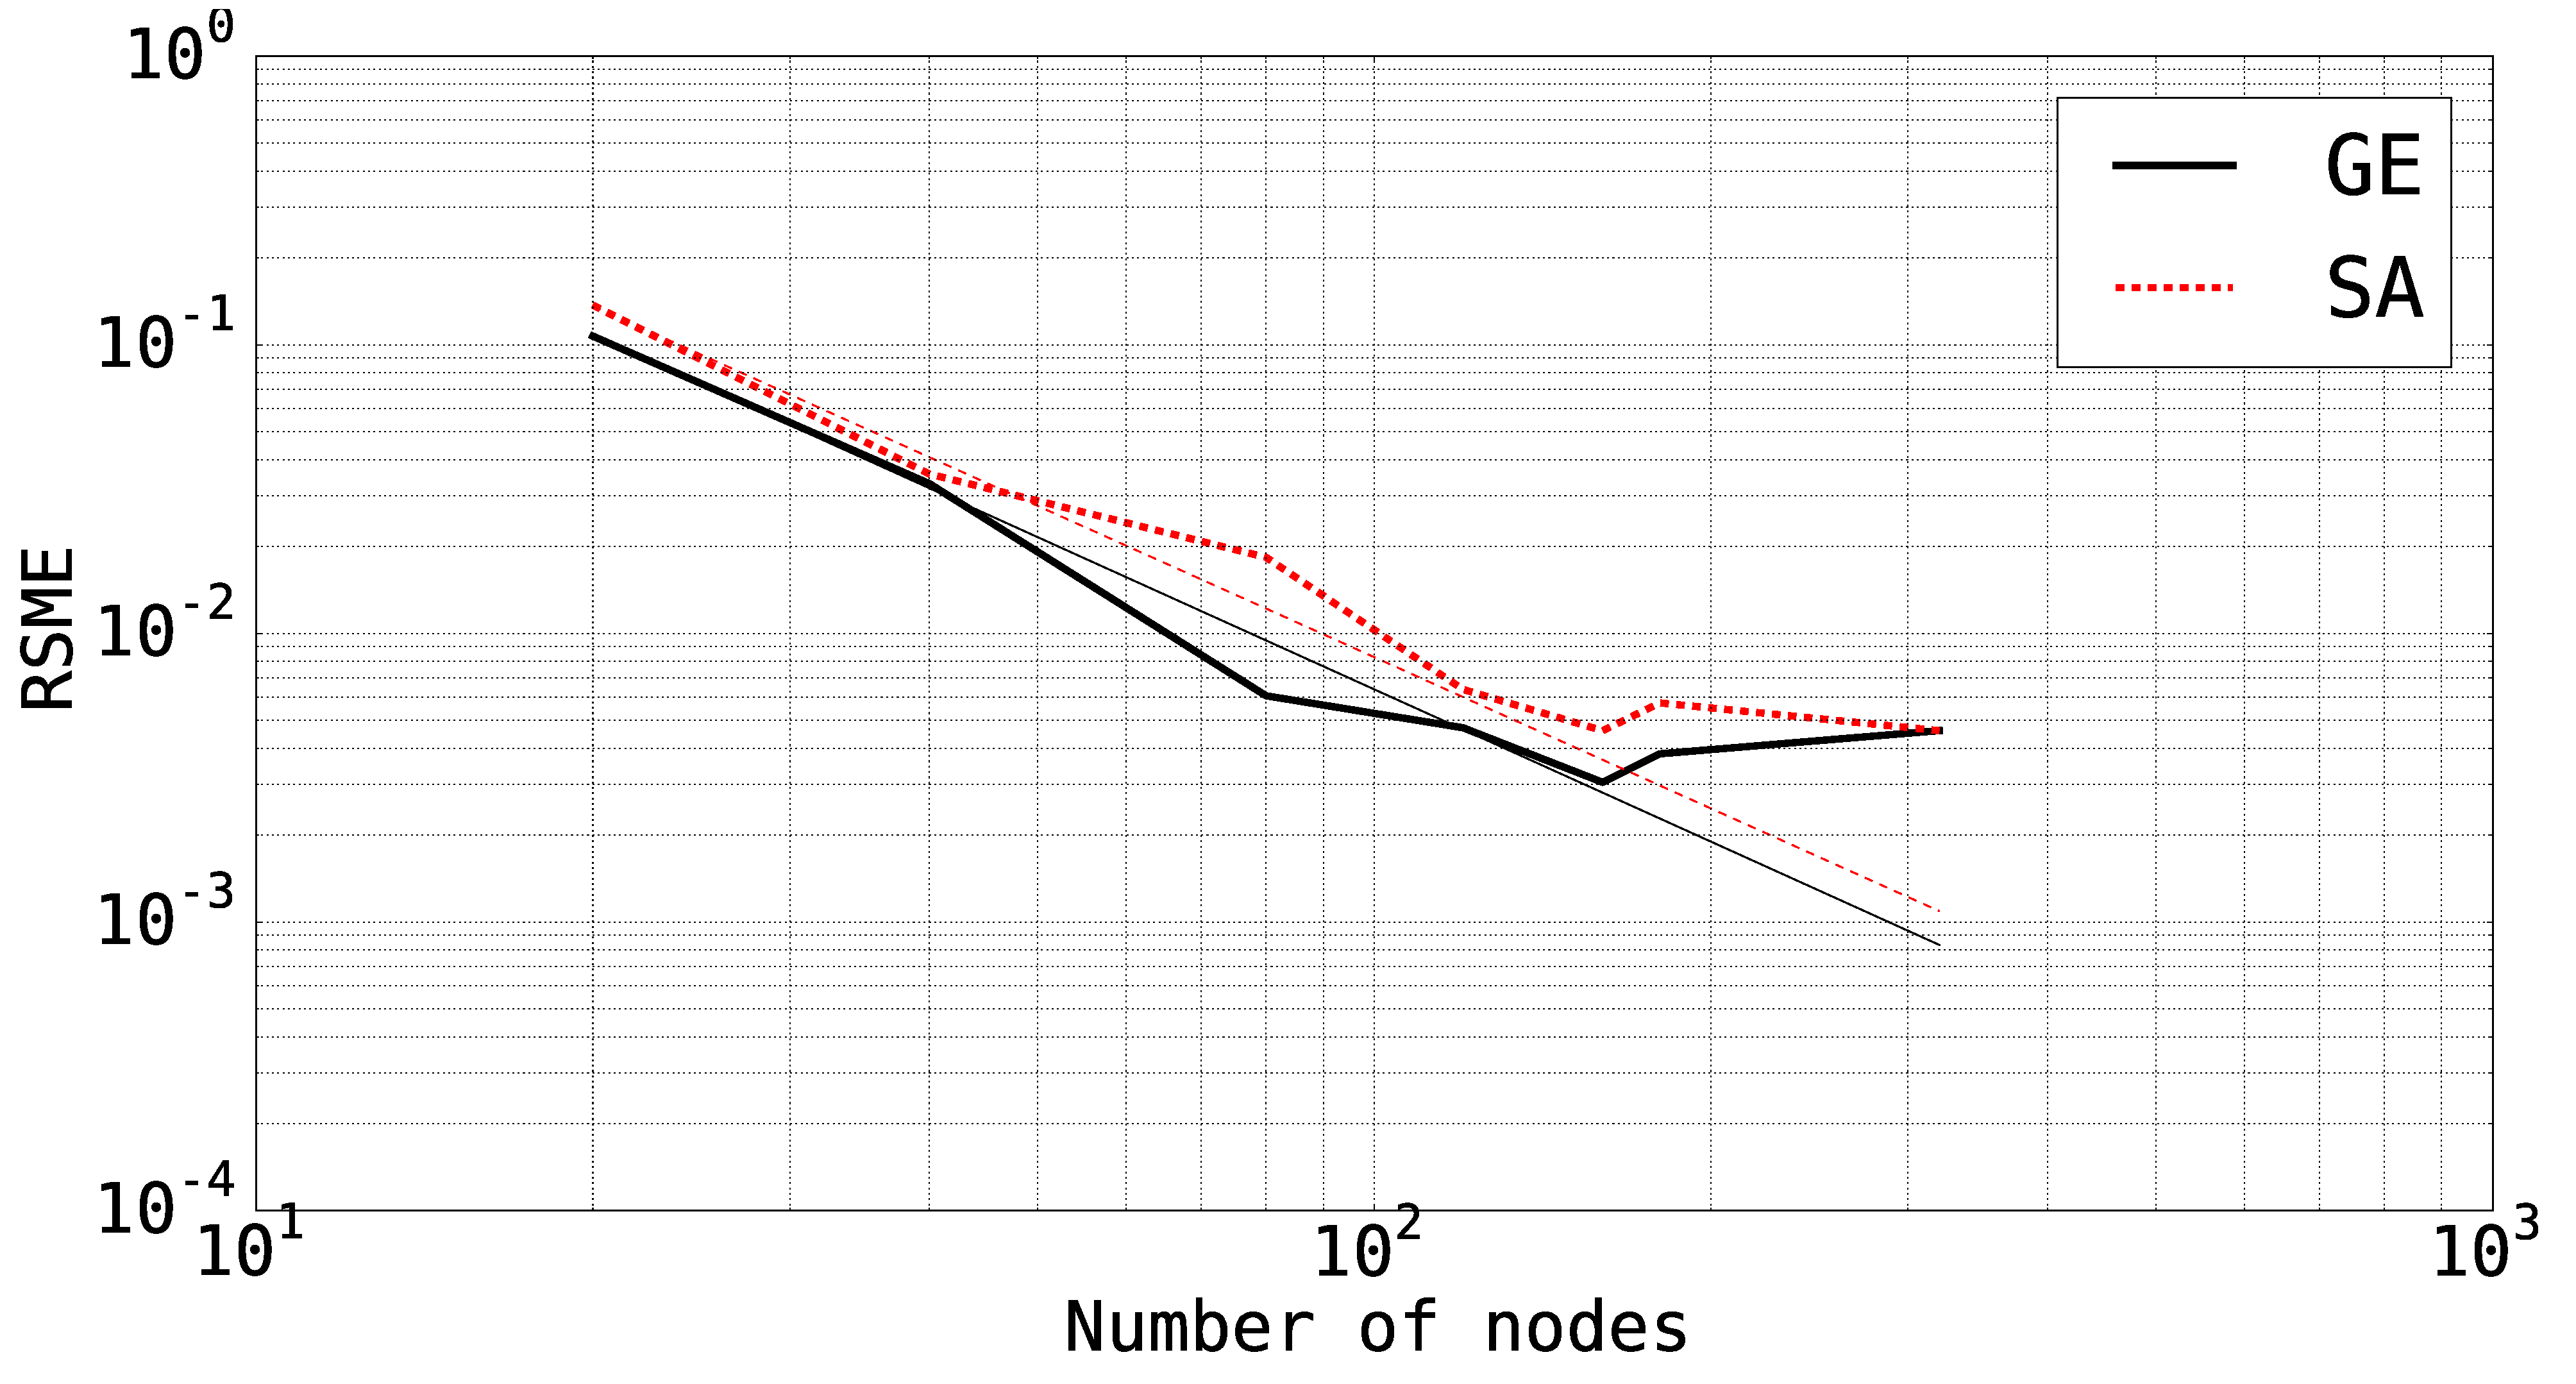
\includegraphics[width=12.0cm]{Chapter_4/figure/penalizationMethod_SA_1D_problem_xw04321.eps}
    }
    \\
    \subfigure[$x_{wall} = 0.7583$]
    {
    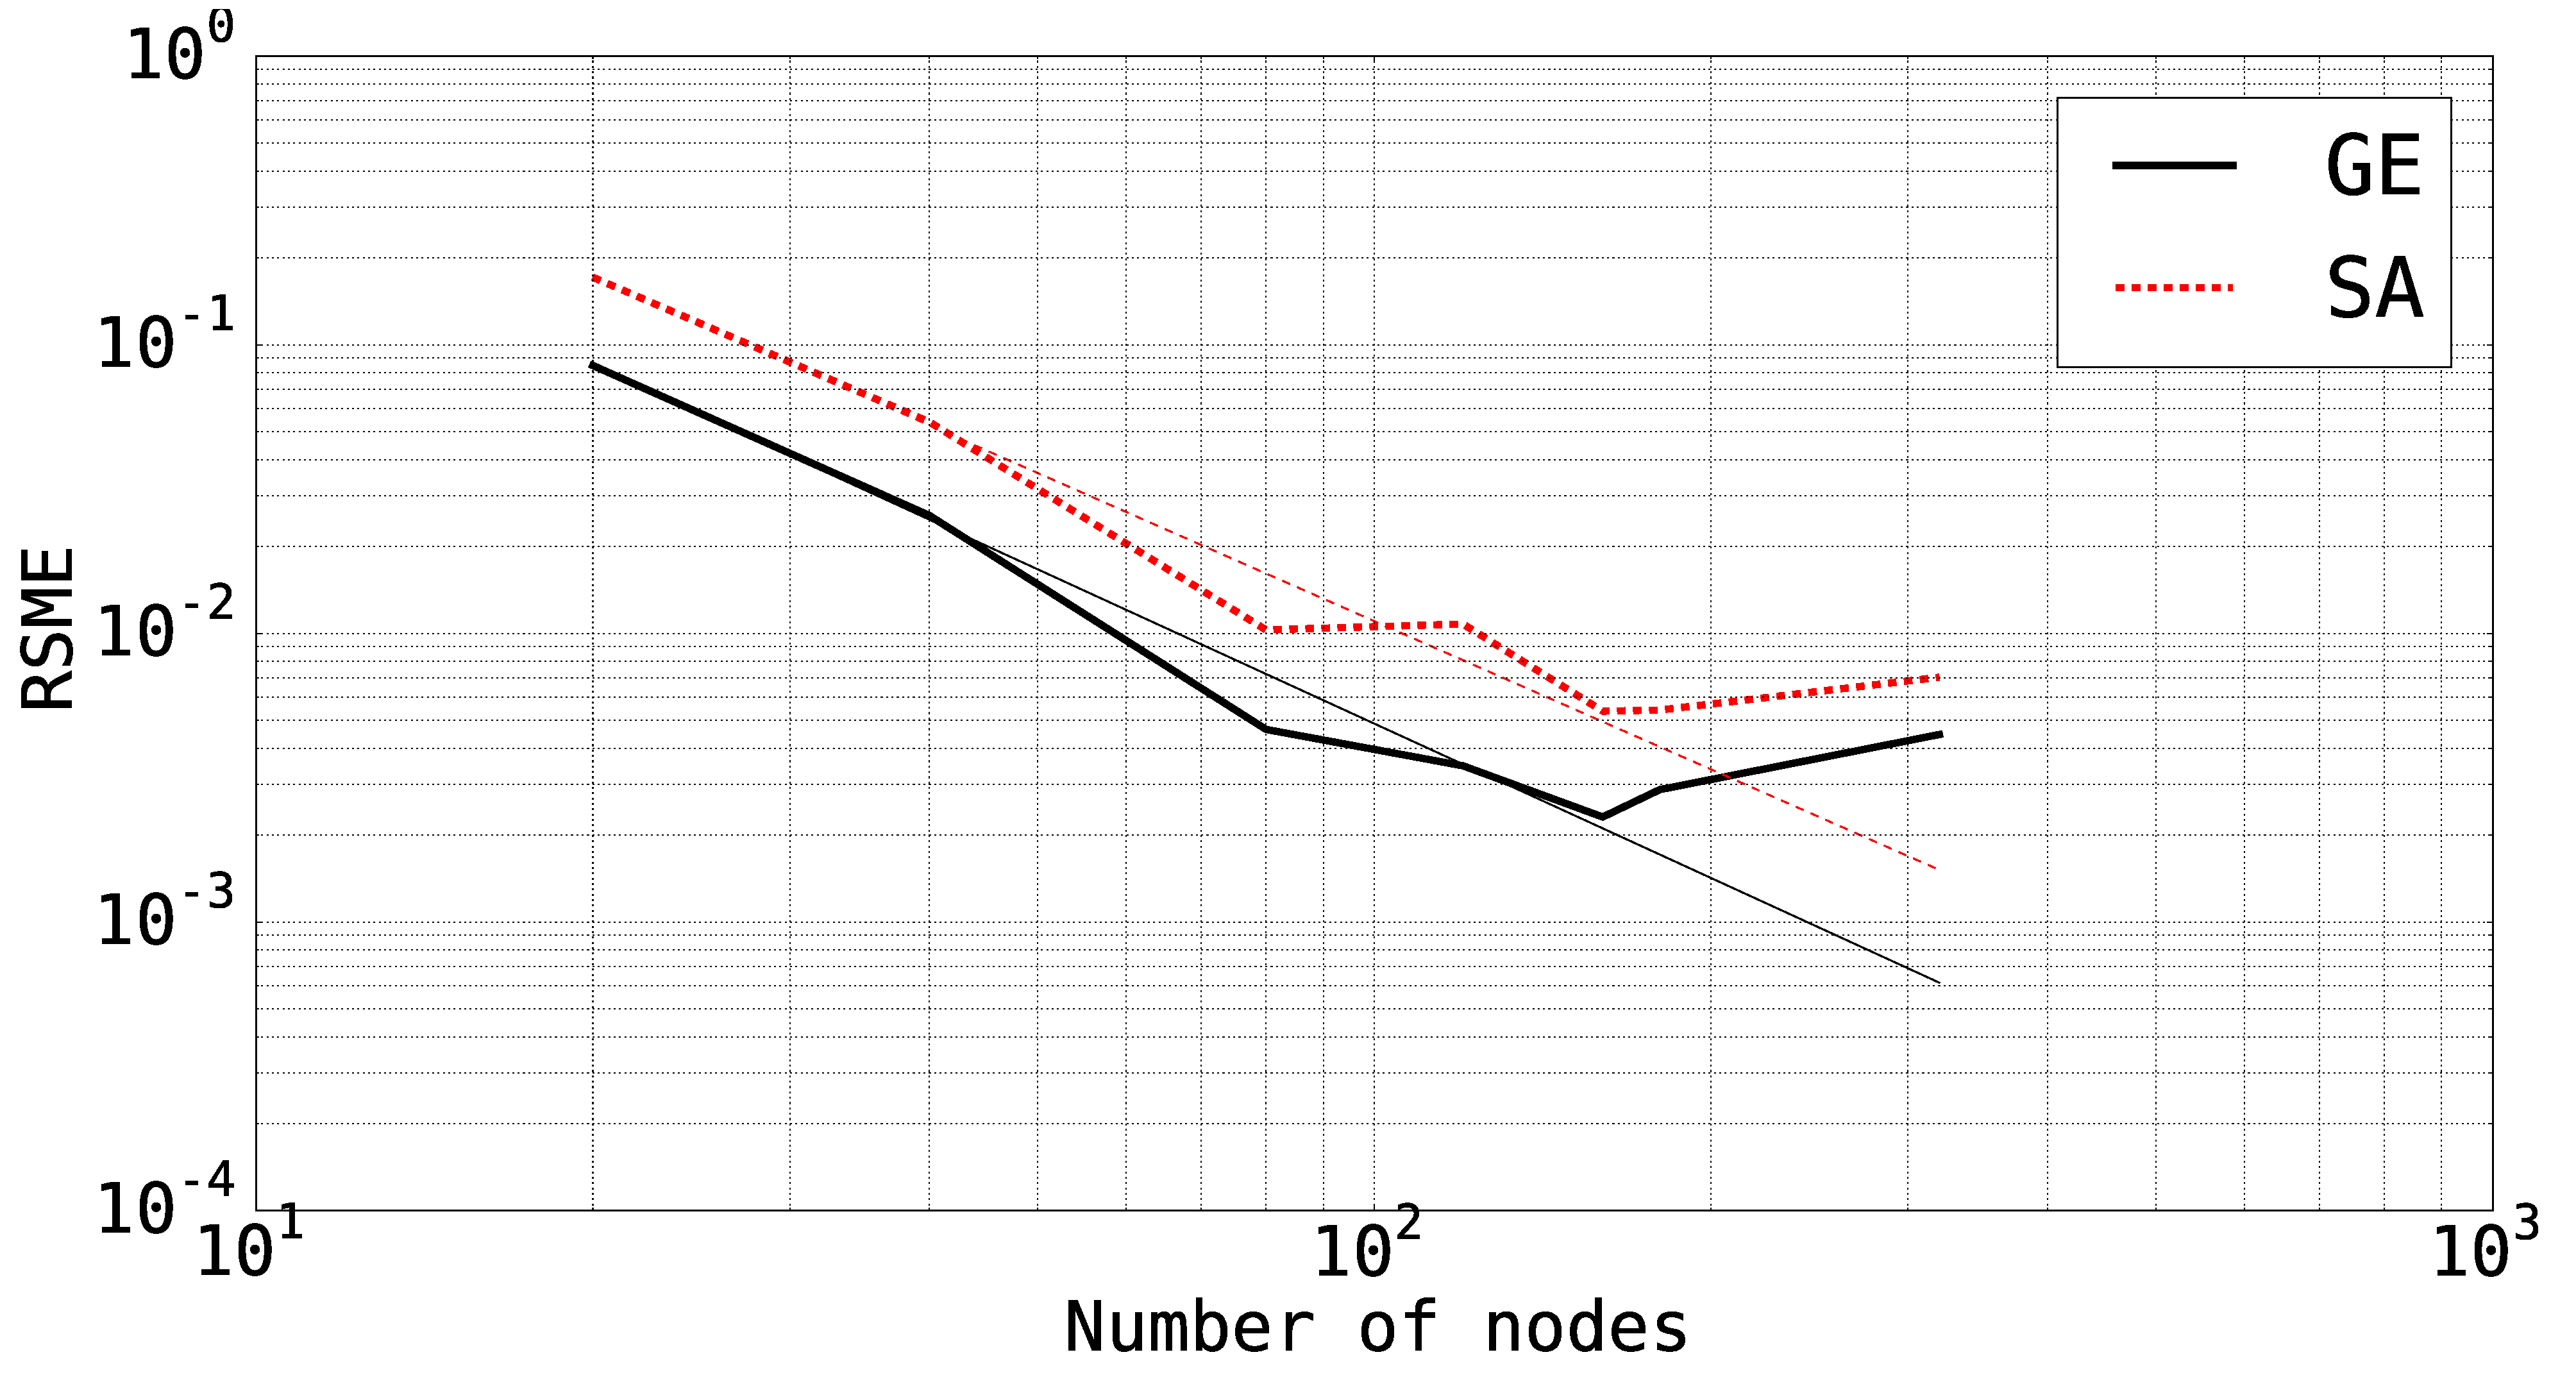
\includegraphics[width=12.0cm]{Chapter_4/figure/penalizationMethod_SA_1D_problem_xw07583.eps}
    }
    \caption{RSME value for the sensitivity analysis (SA) and governing equation (GE).}
    \label{fig:C4_effectOfNumberOfNodesOnSensitivityResults1Dproblem}
\end{figure}

The thin lines in Figure \ref{fig:C4_effectOfRHfunctionOnSimulationResults1Dproblem}, represents the curve fit by function $y = ae^{bx}$ through the RSME values. The slope of this line is $-1.75$ for both of these analysis. This means that the rate of convergence is the same for governing equations and sensitivity analysis for this problem. The source of the error between the analytical and the CSA is better investigated by looking at the comparison between the sensitivity of the velocity profile to the distance between the plates as shown in Figure \ref{fig:C4_sensitivityResults1Dproblem}.

\begin{figure}[H]
    \centering
    \subfigure[$x_{wall} = 0.4321, n = 120$]
    {
    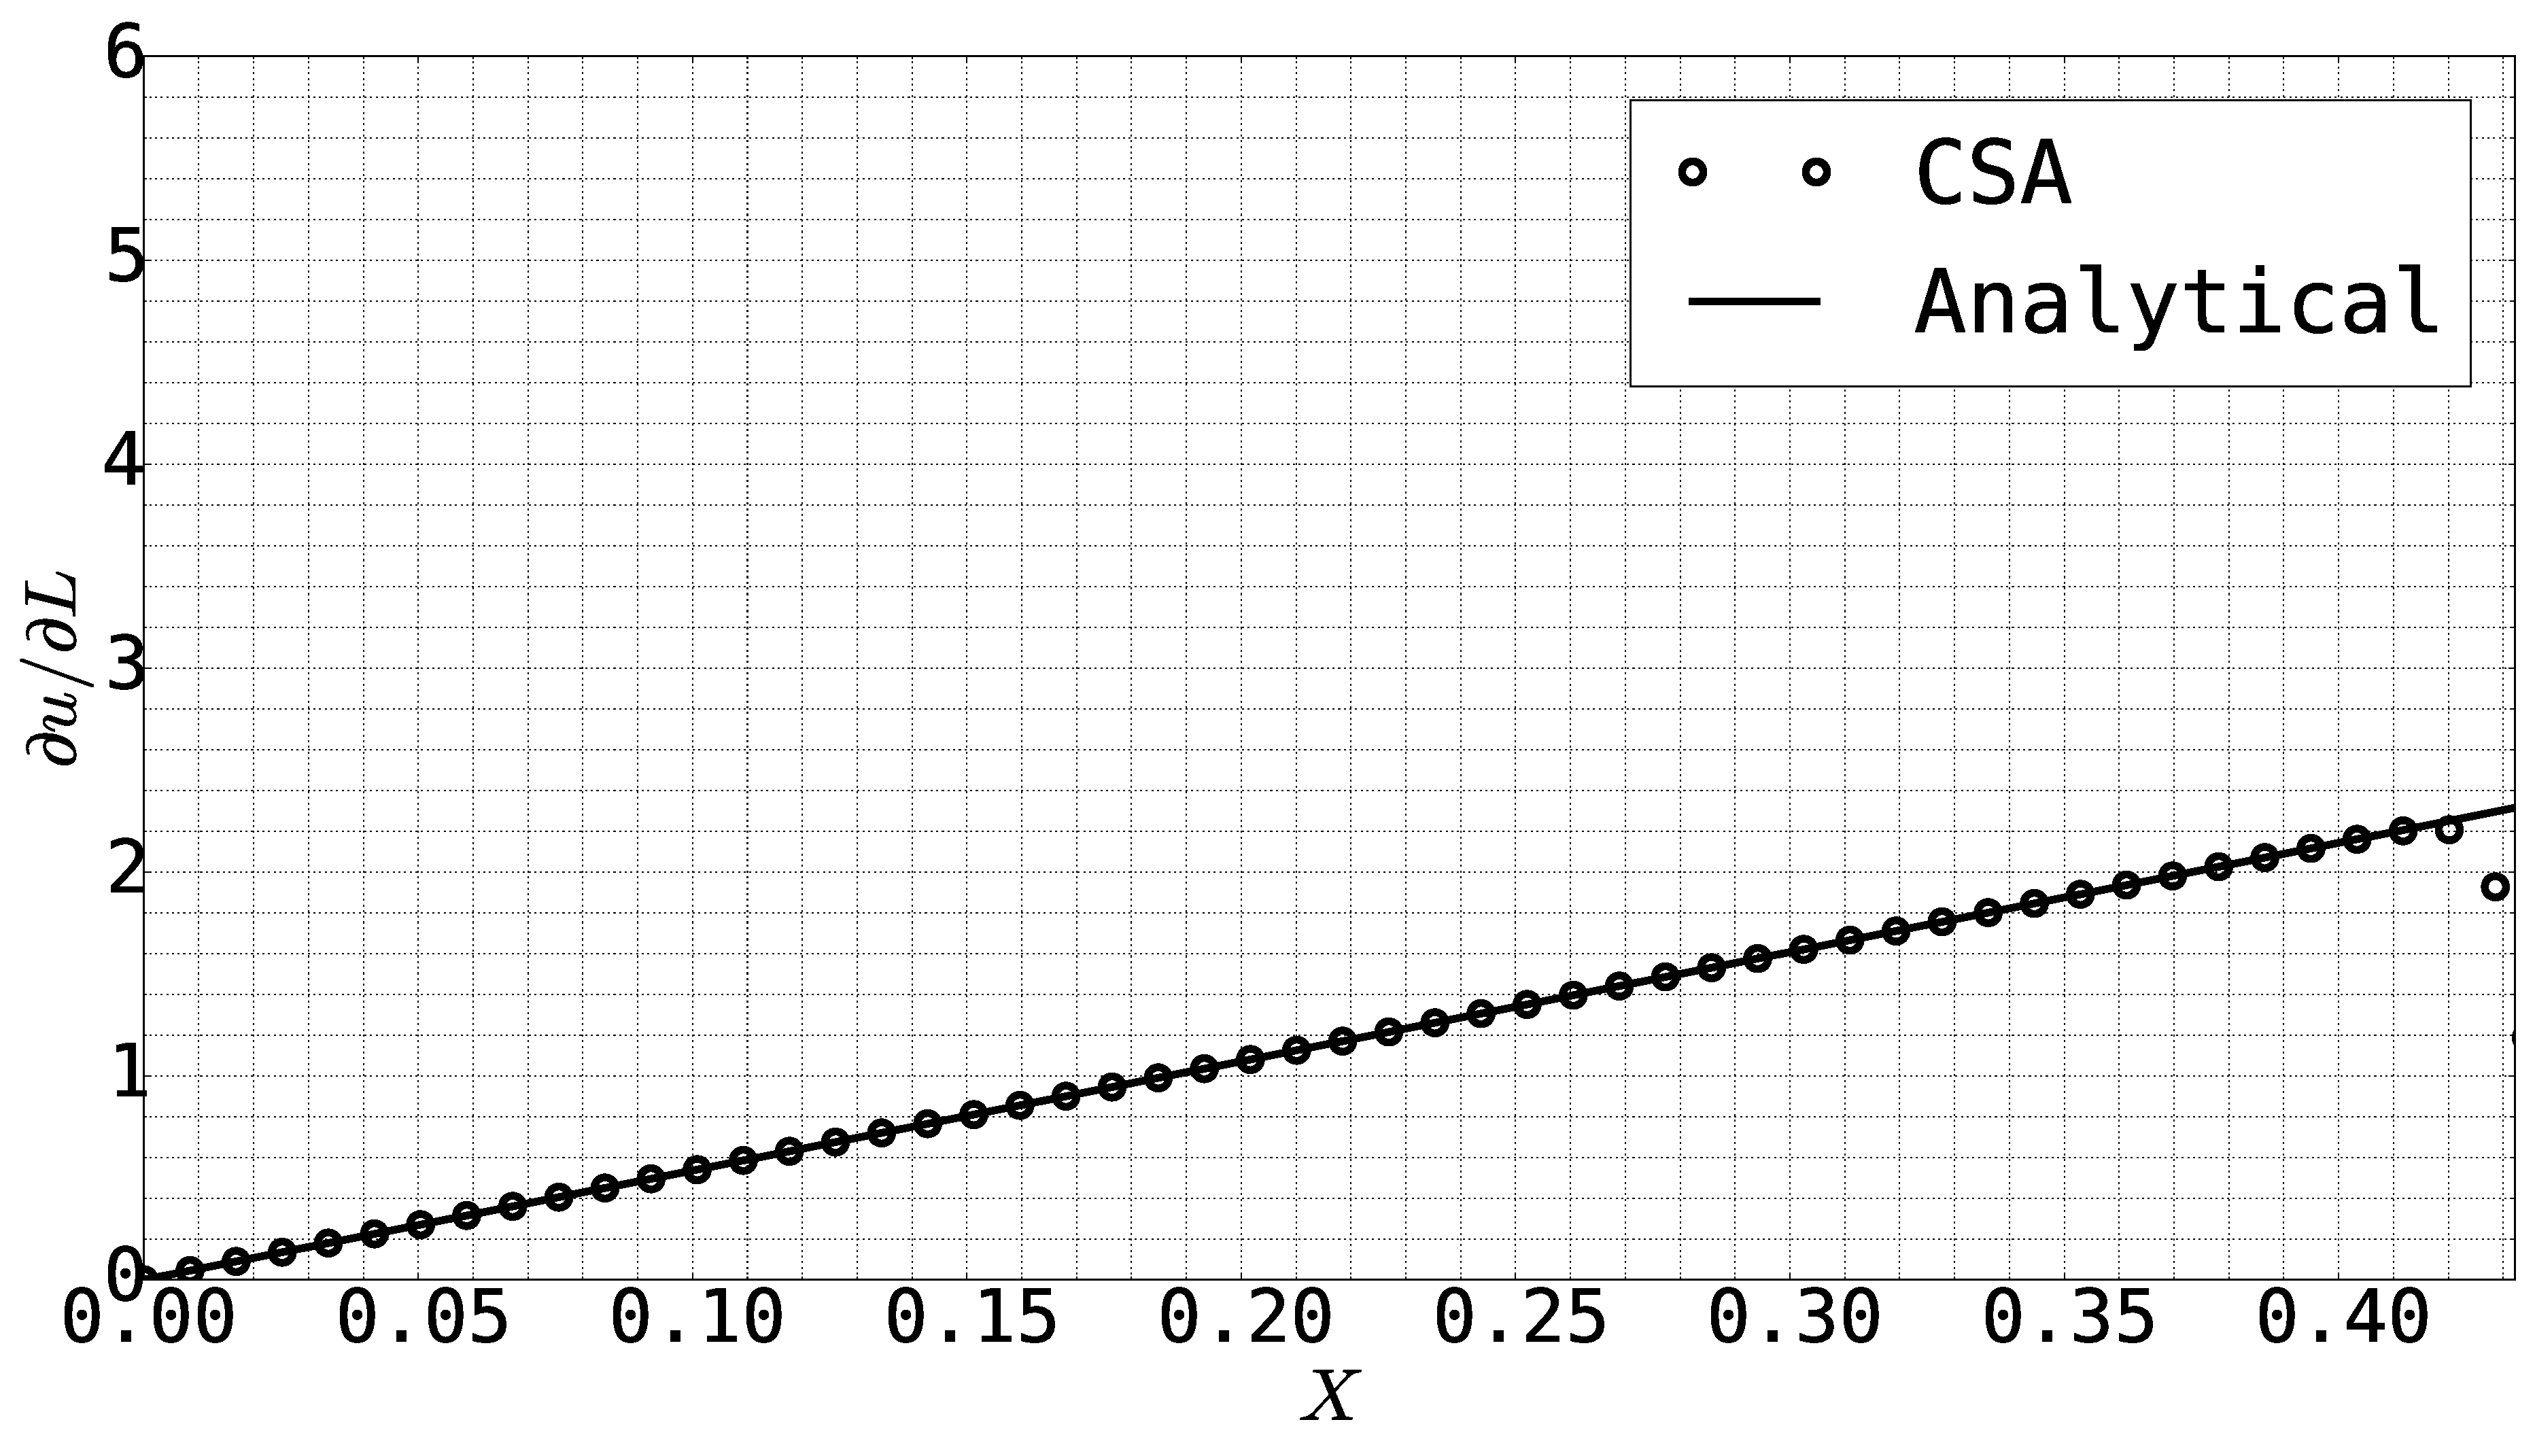
\includegraphics[width=7.0cm]{Chapter_4/figure/penalizationMethod_sensitivityProfile_xw04321.eps}
    }
    \quad
    \subfigure[$x_{wall} = 0.7583, n = 120$]
    {
    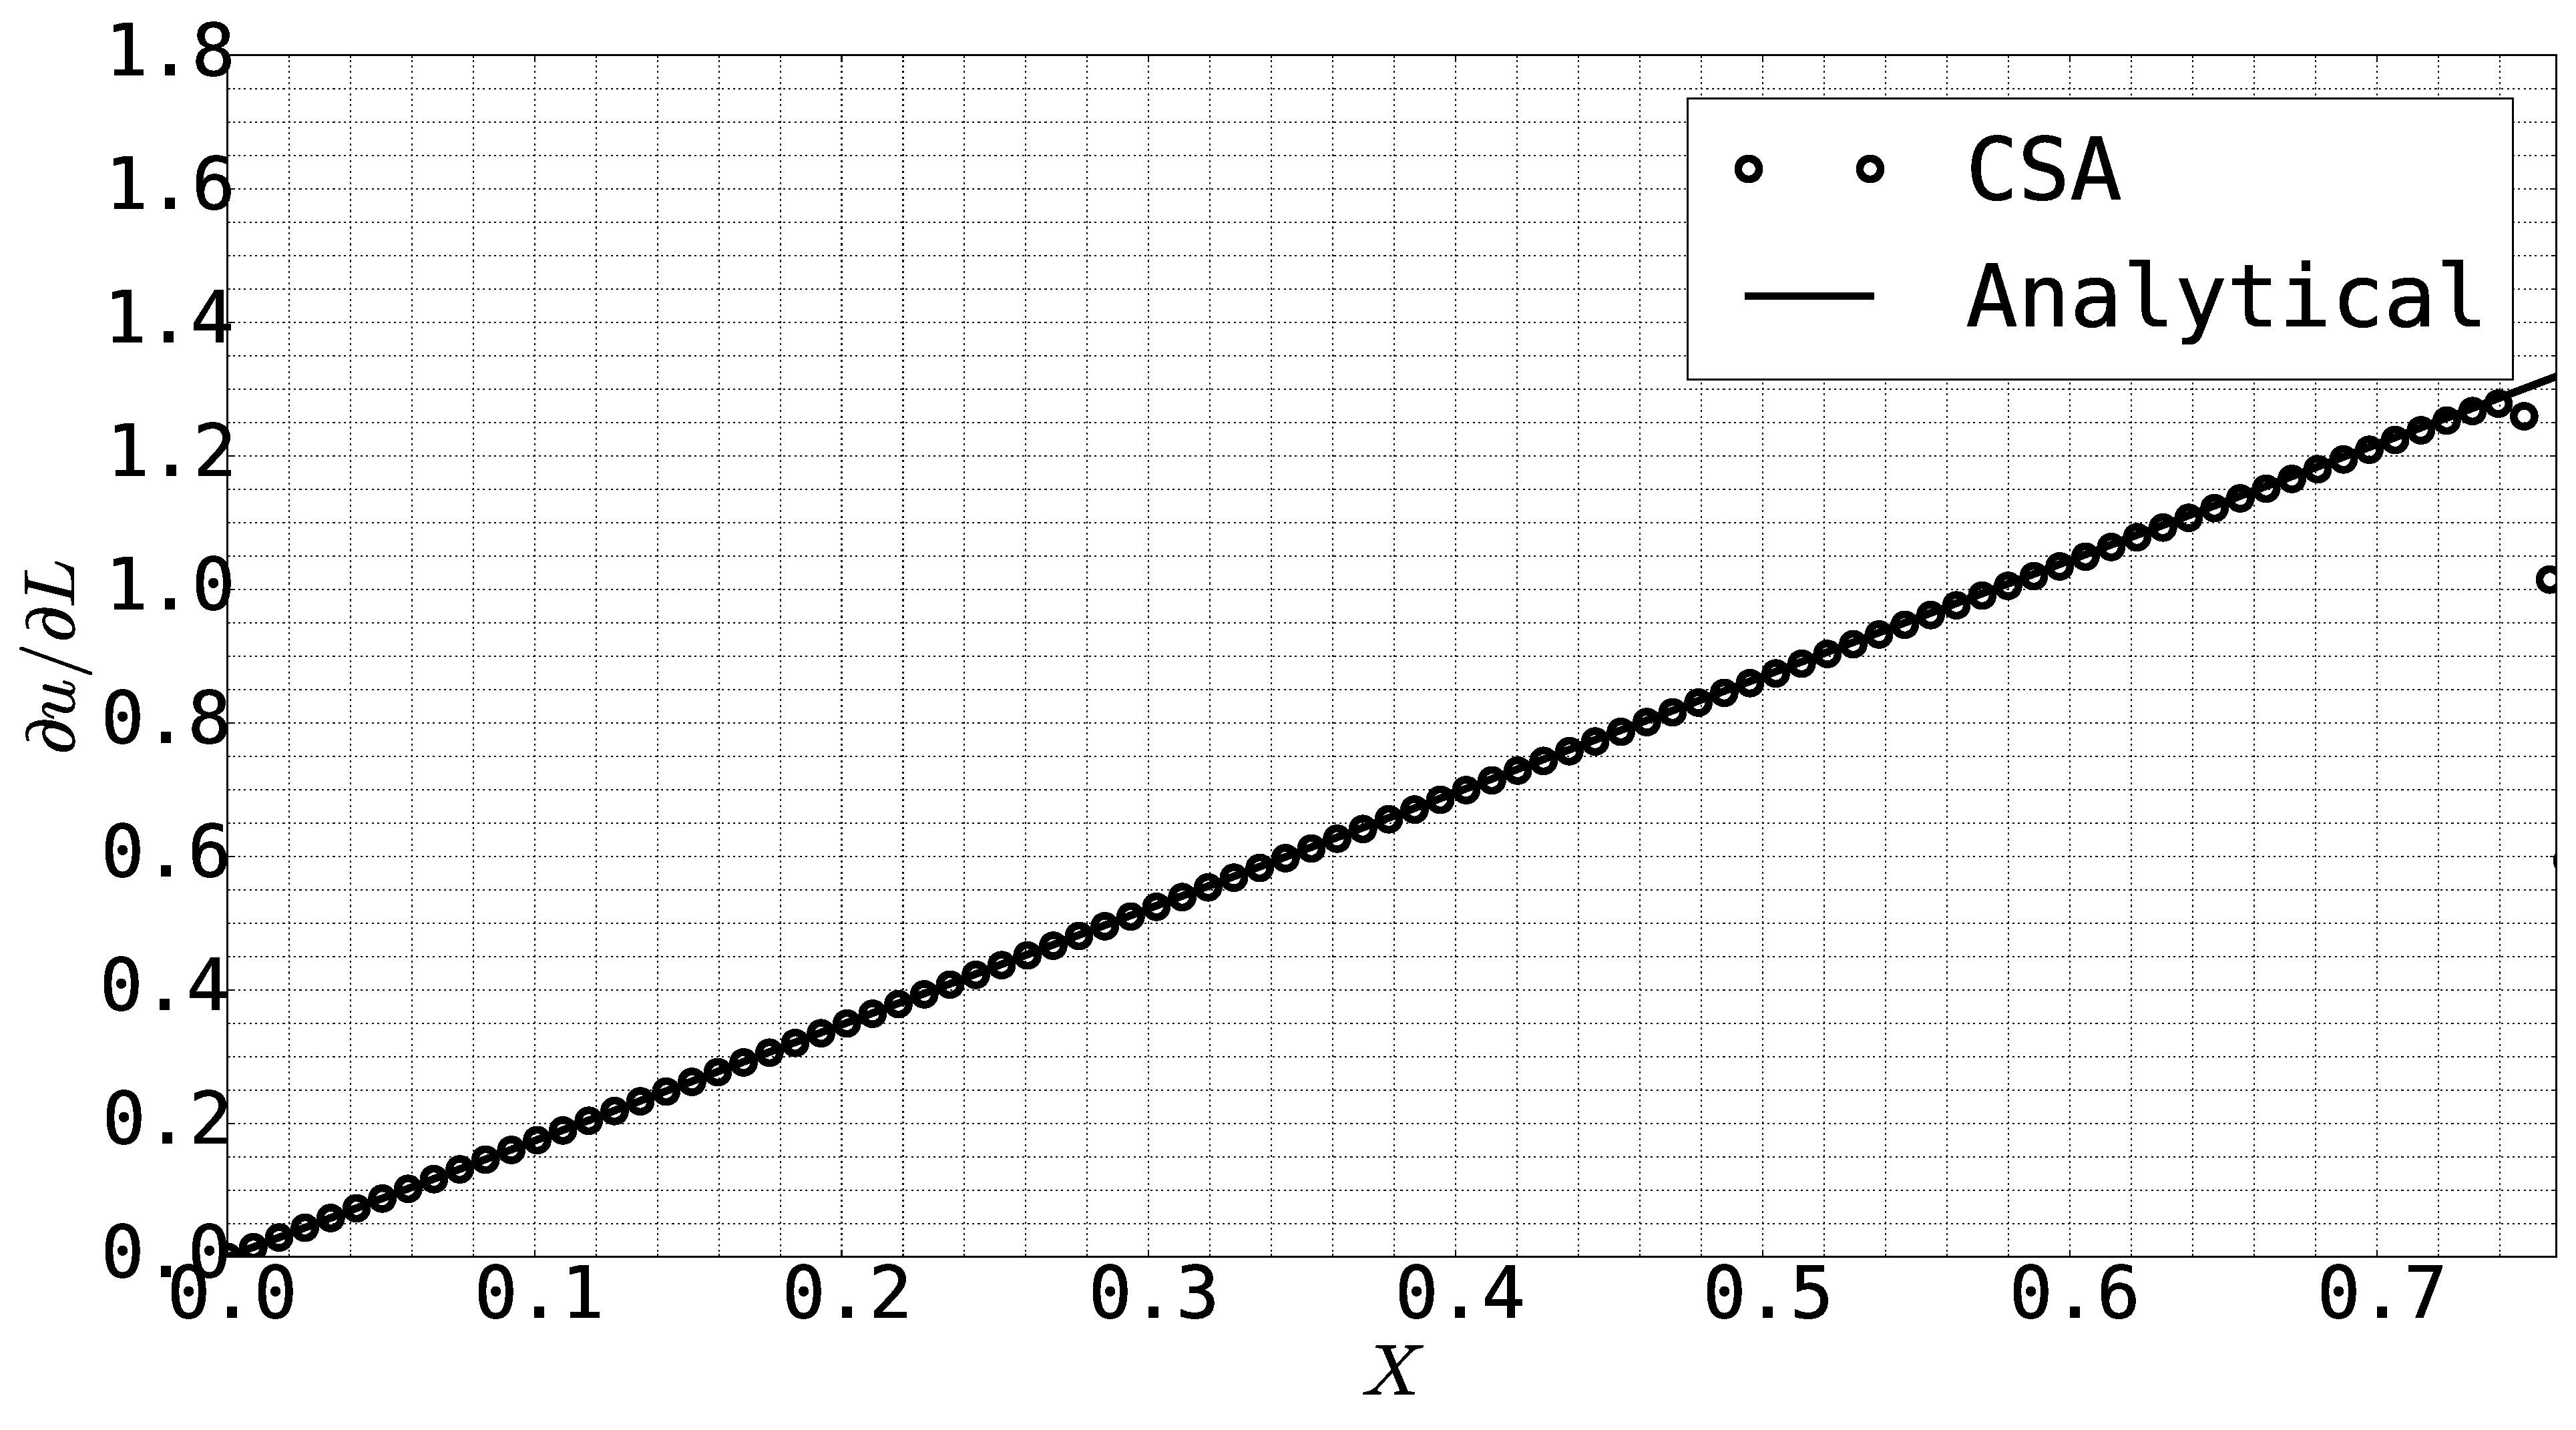
\includegraphics[width=7.0cm]{Chapter_4/figure/penalizationMethod_sensitivityProfile_xw07583.eps}
    }
    \\
    \subfigure[$x_{wall} = 0.2451, n = 30$]
    {
    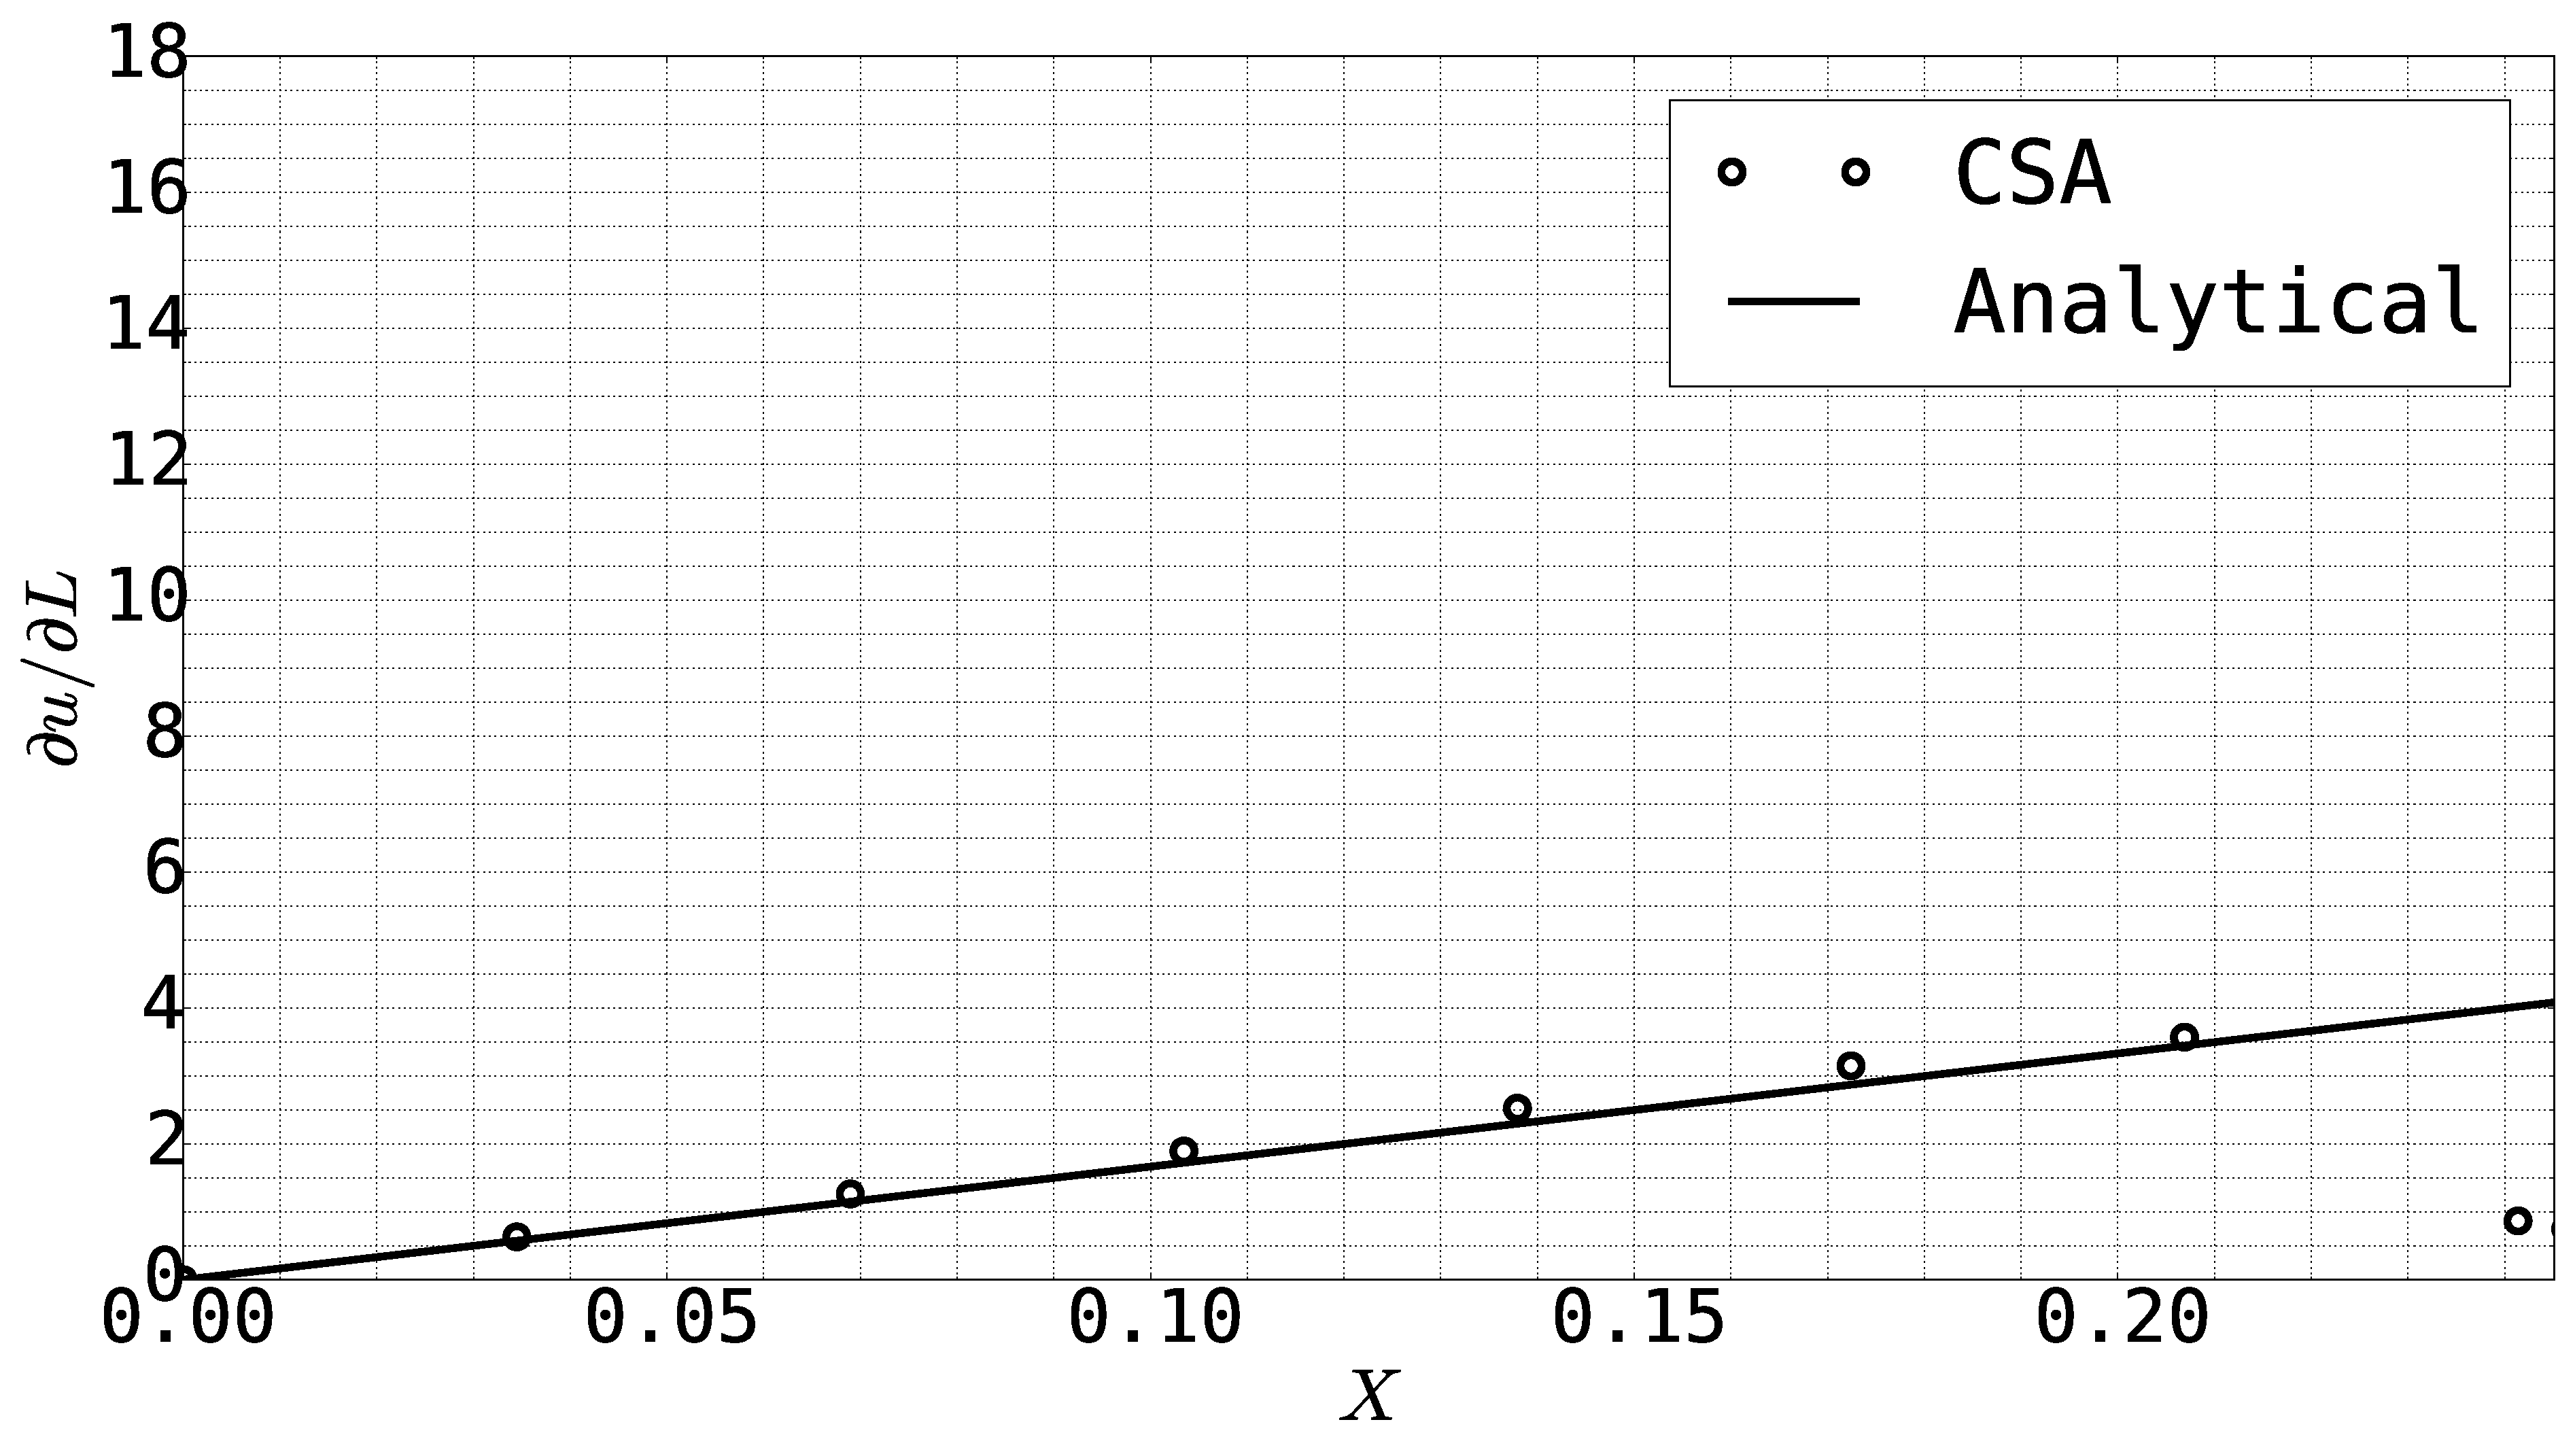
\includegraphics[width=7.0cm]{Chapter_4/figure/penalizationMethod_sensitivityProfile_xw02451.eps}
    }
    \quad
    \subfigure[$x_{wall} = 0.5742, n = 60$]
    {
    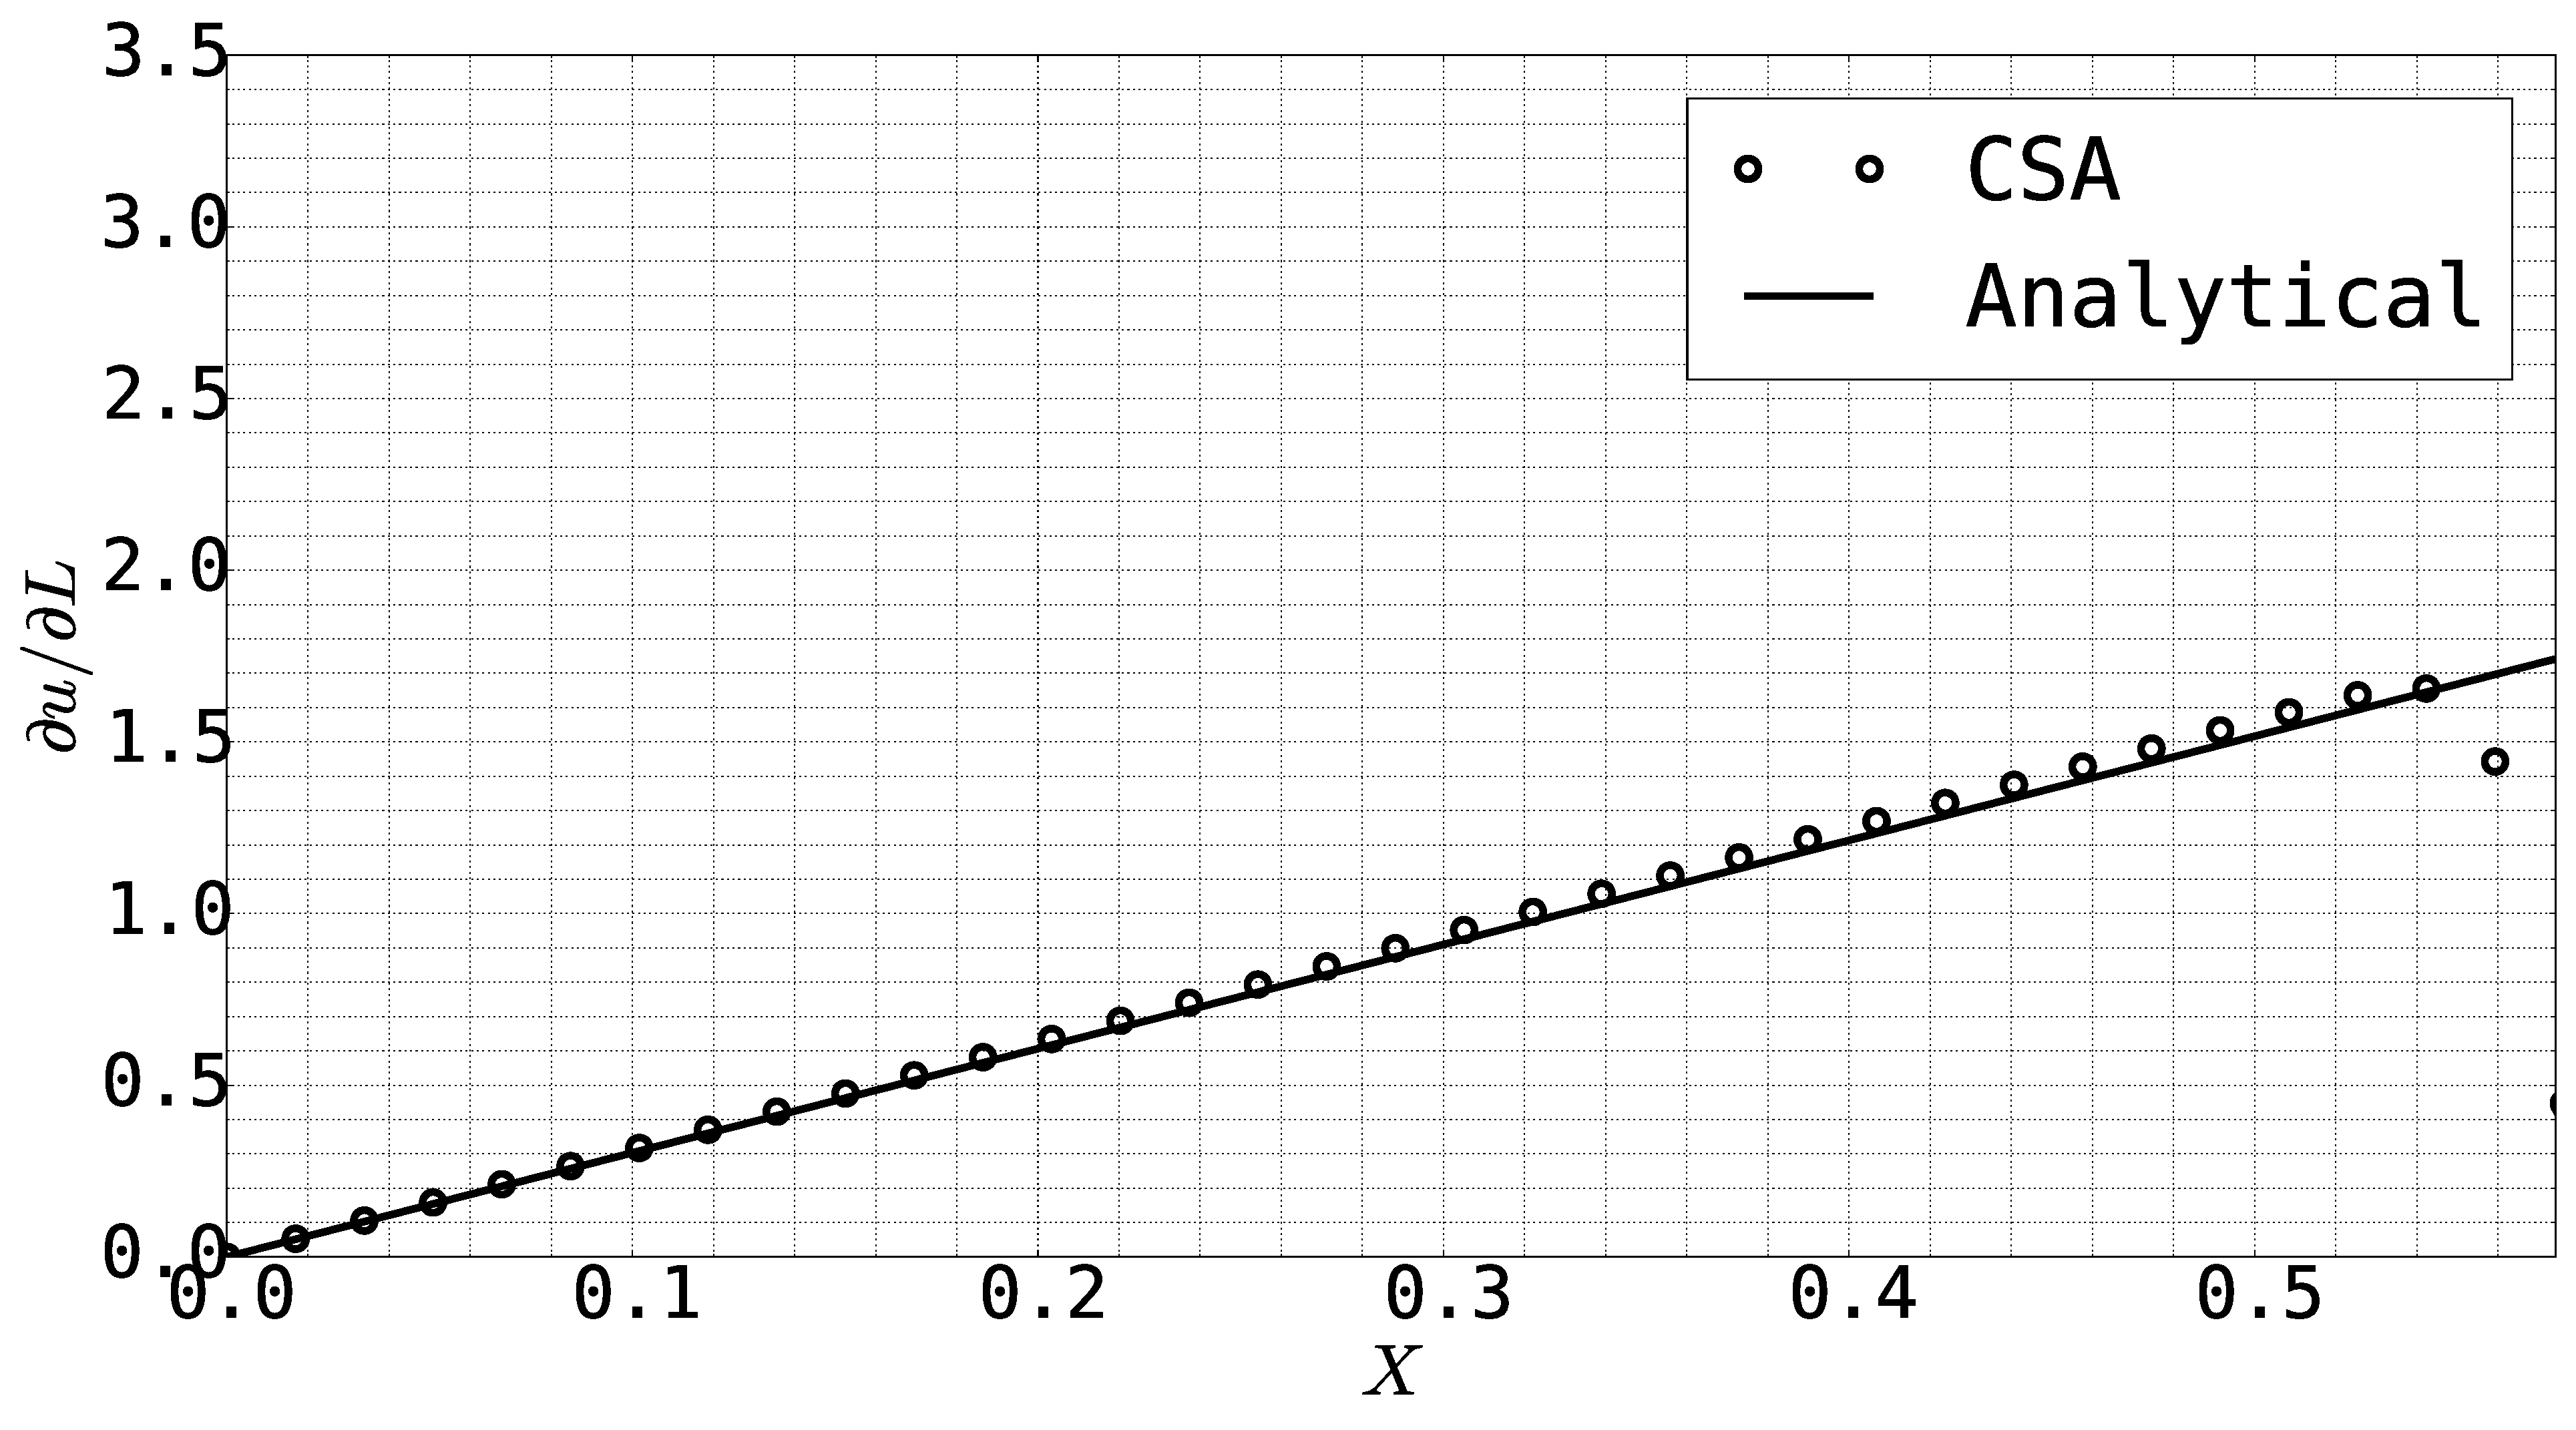
\includegraphics[width=7.0cm]{Chapter_4/figure/penalizationMethod_sensitivityProfile_xw05742.eps}
    }
    \caption{Comparison between the velocity sensitivity profile of CSA and analytical results in the domain. $w_{wall}$ is the location of the stationary wall and $n$ is the number of nodes used to discretize the domain.}
    \label{fig:C4_sensitivityResults1Dproblem}
\end{figure}

As shown in Figure \ref{fig:C4_sensitivityResults1Dproblem}, the accuracy of CSA results start to decay near the boundary. It should be noted that this domain corresponds to the region that we chose the RH function value to have its 99 percent change in. Therefore, the size of this region is known before the analysis. As shown in Figure \ref{fig:C4_sensitivityResults1Dproblem}, did not affect the sensitivity results in regions further away from the boundary. This means that the sensitivities near the boundary can be reconstructed by post-processing the sensitivity data. This is done using function approximation techniques such as linear extrapolation or TANA \cite{wang1995improved}. The reconstructed results of Figure \ref{fig:C4_sensitivityResults1Dproblem} using linear extrapolation are shown in Figure \ref{fig:C4_sensitivityResultsReconstructed1Dproblem}.

\begin{figure}[H]
    \centering
    \subfigure[$x_{wall} = 0.4321, n = 120$]
    {
    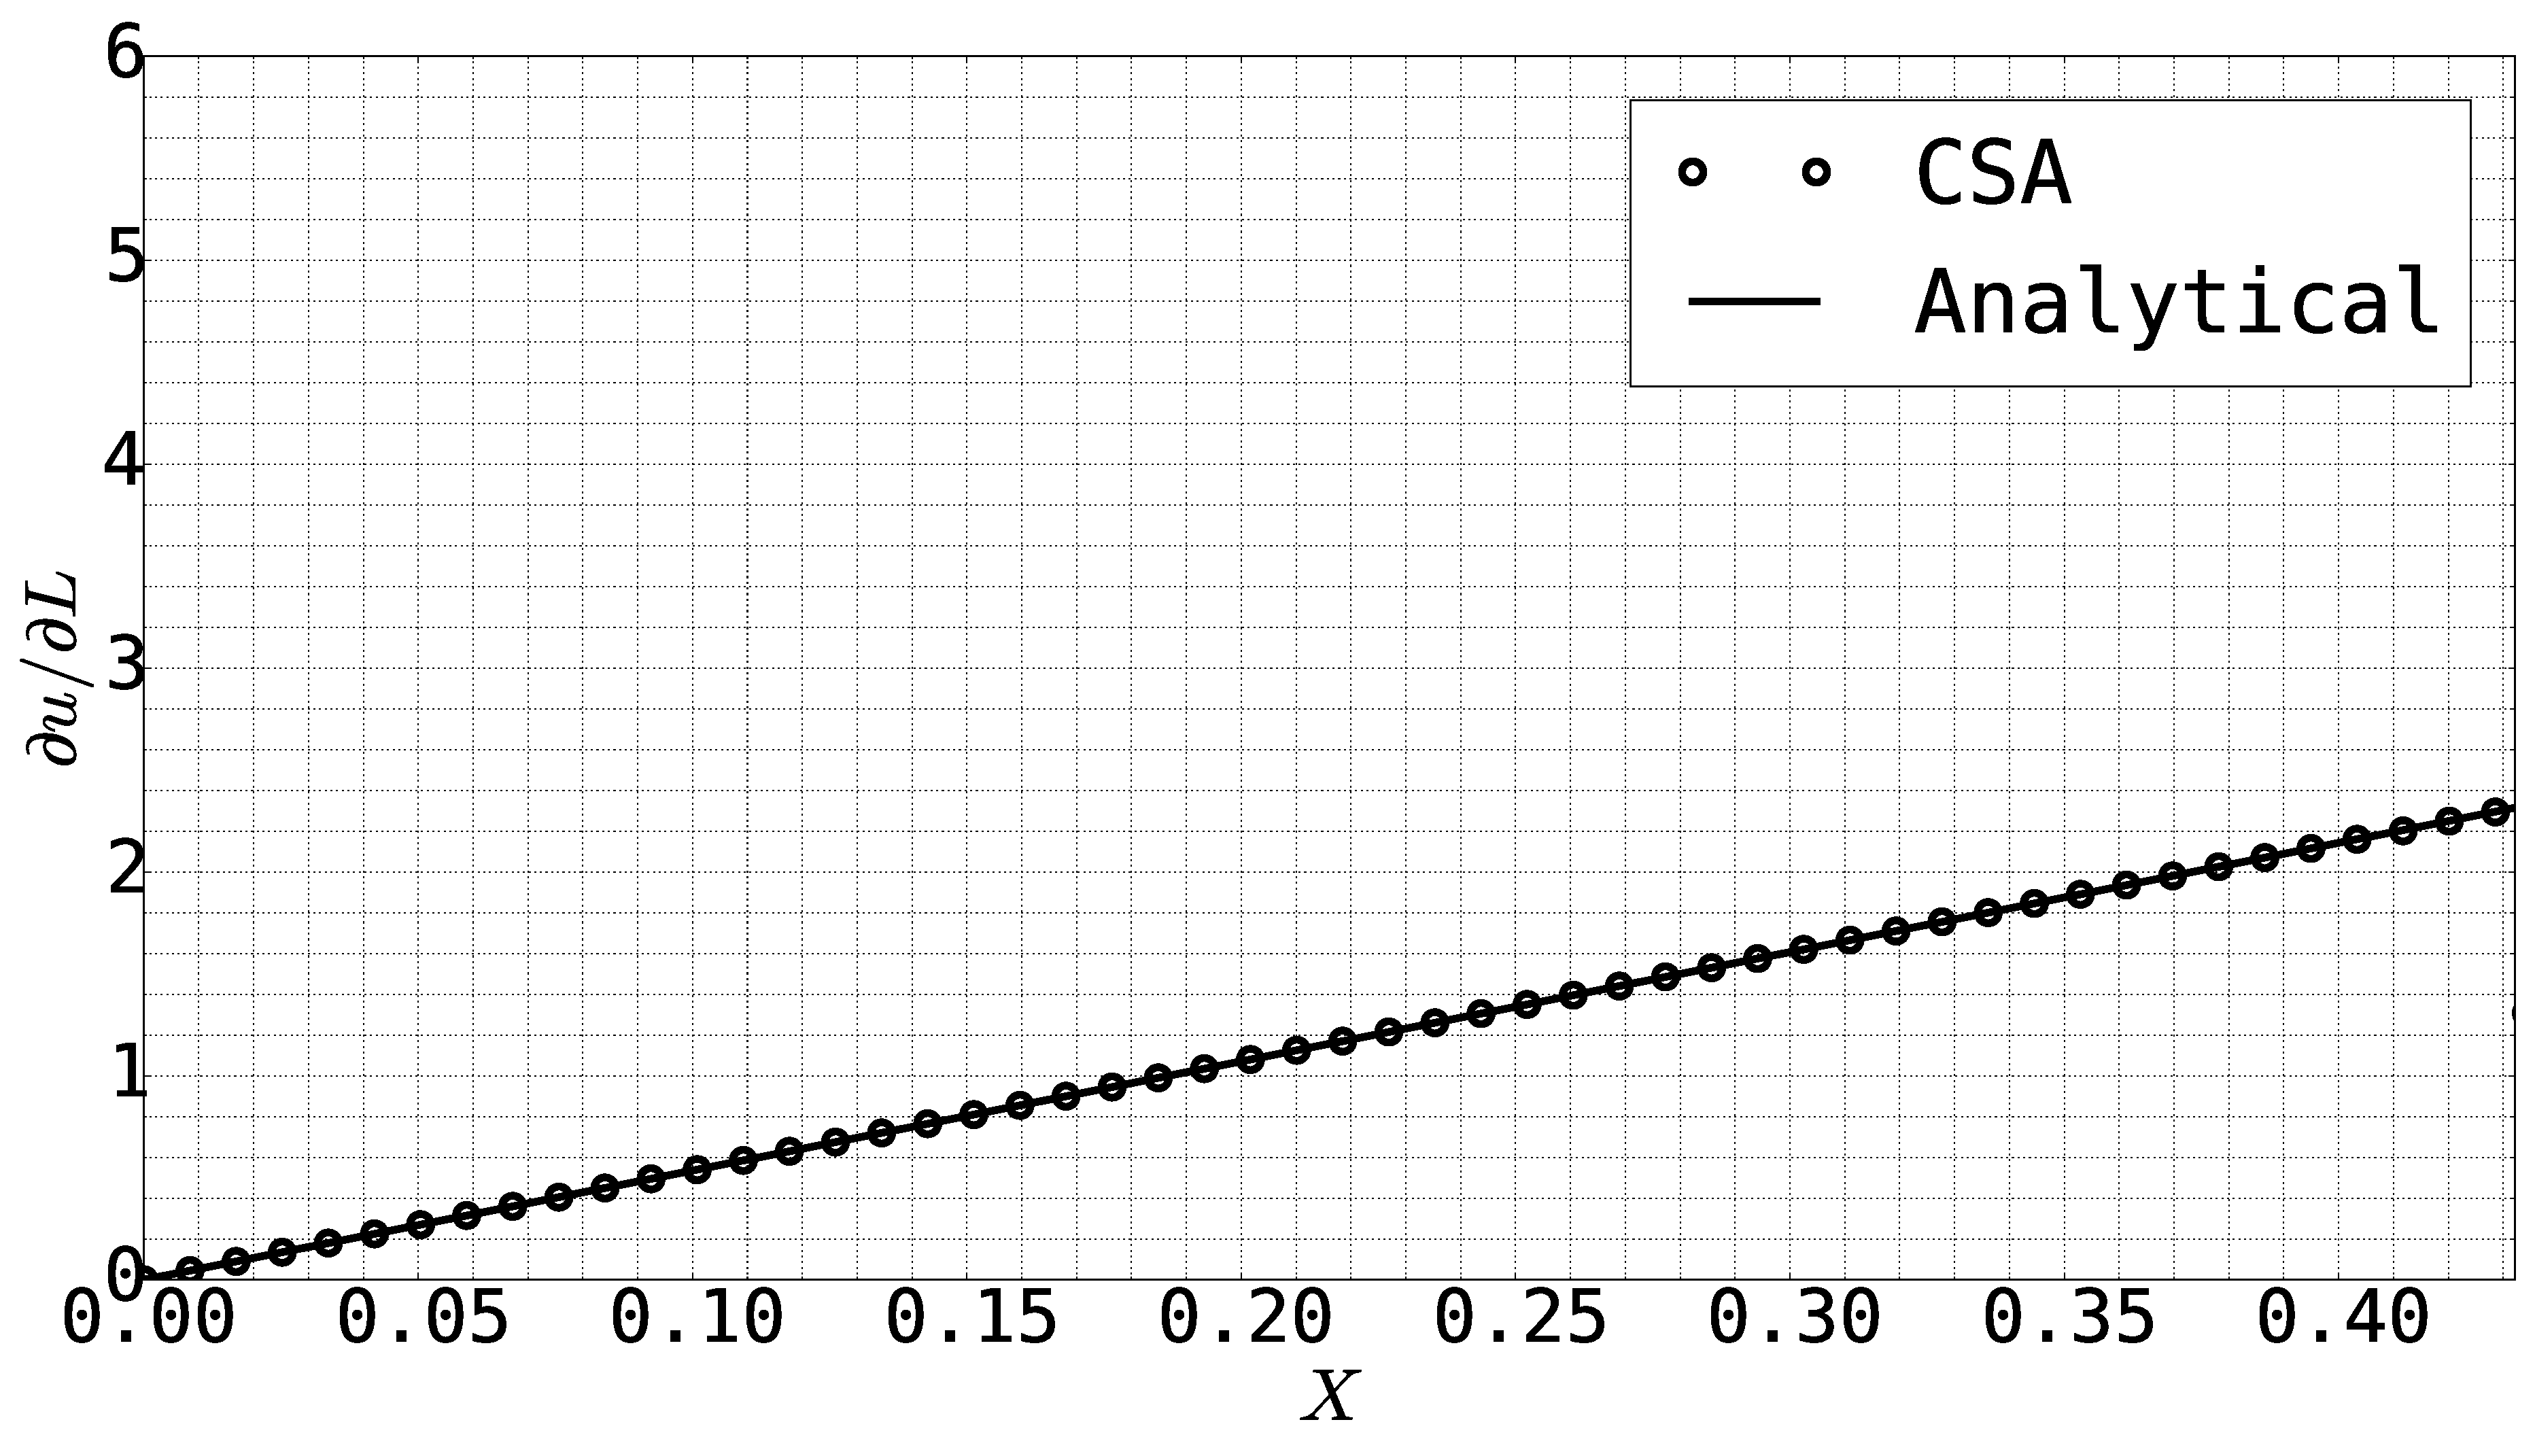
\includegraphics[width=7.0cm]{Chapter_4/figure/penalizationMethod_sensitivityProfile_reconstructed_xw04321.eps}
    }
    \quad
    \subfigure[$x_{wall} = 0.7583, n = 120$]
    {
    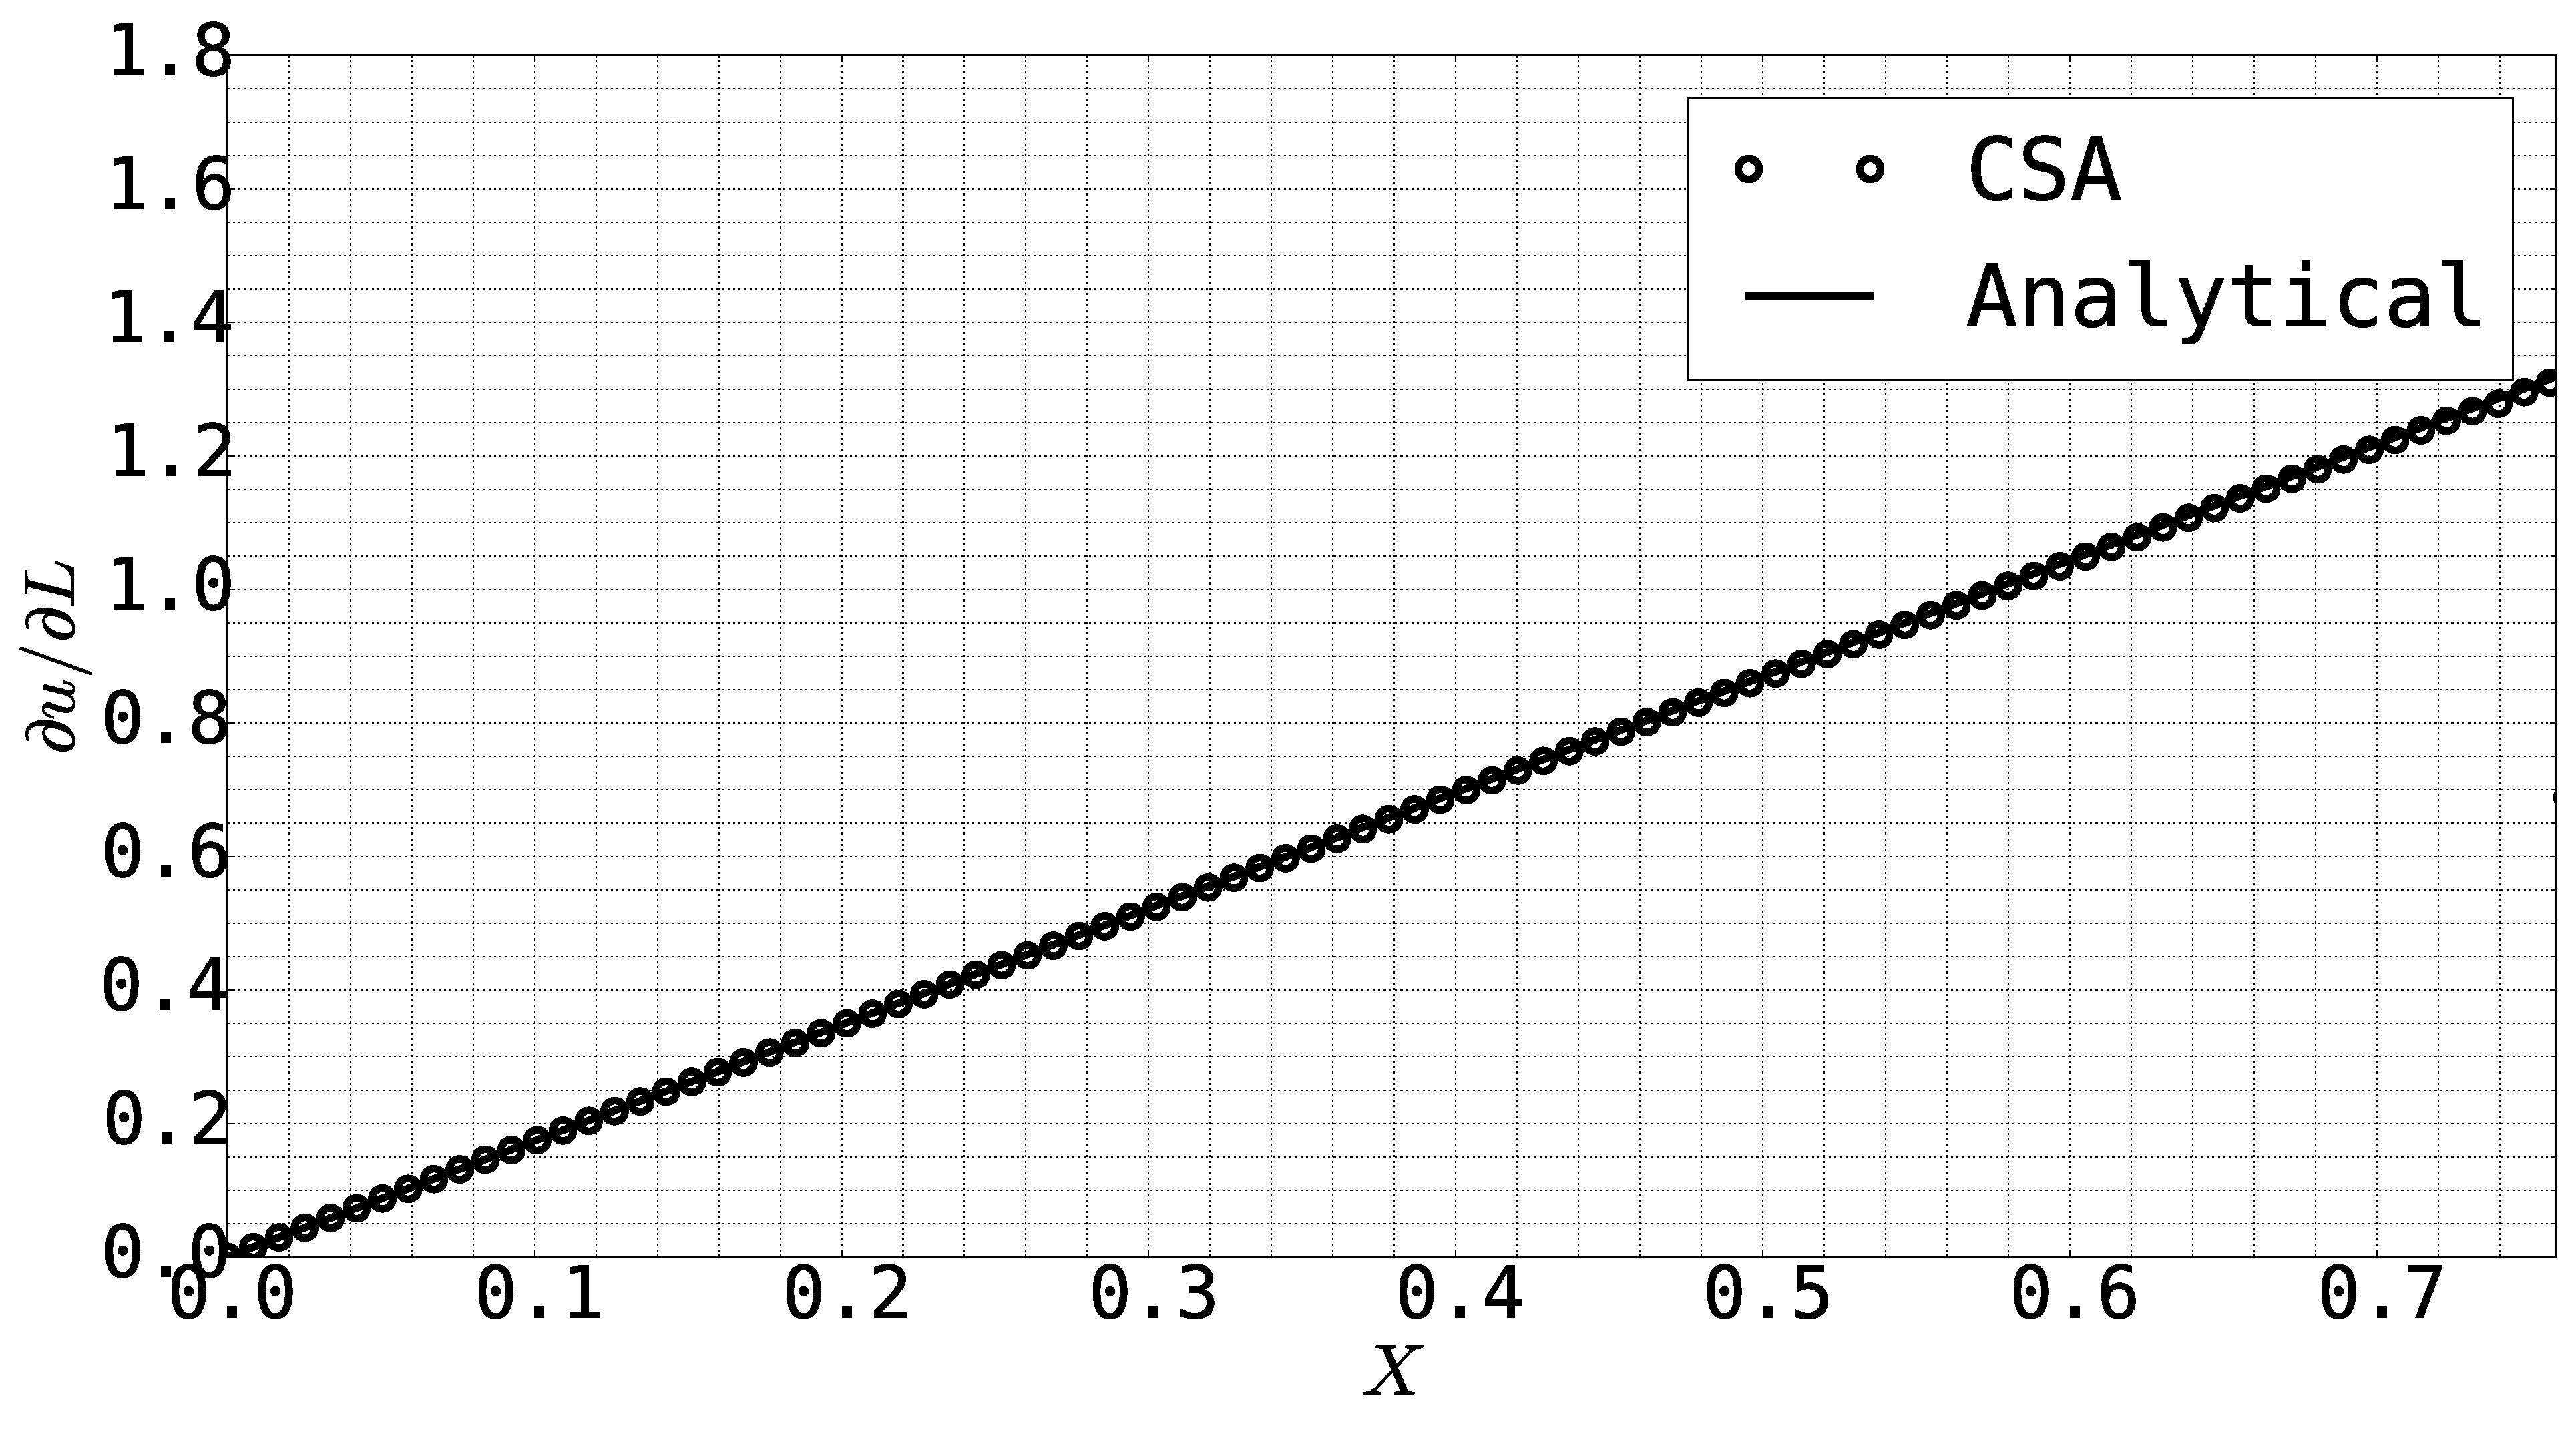
\includegraphics[width=7.0cm]{Chapter_4/figure/penalizationMethod_sensitivityProfile_reconstructed_xw07583.eps}
    }
    \\
    \subfigure[$x_{wall} = 0.2451, n = 30$]
    {
    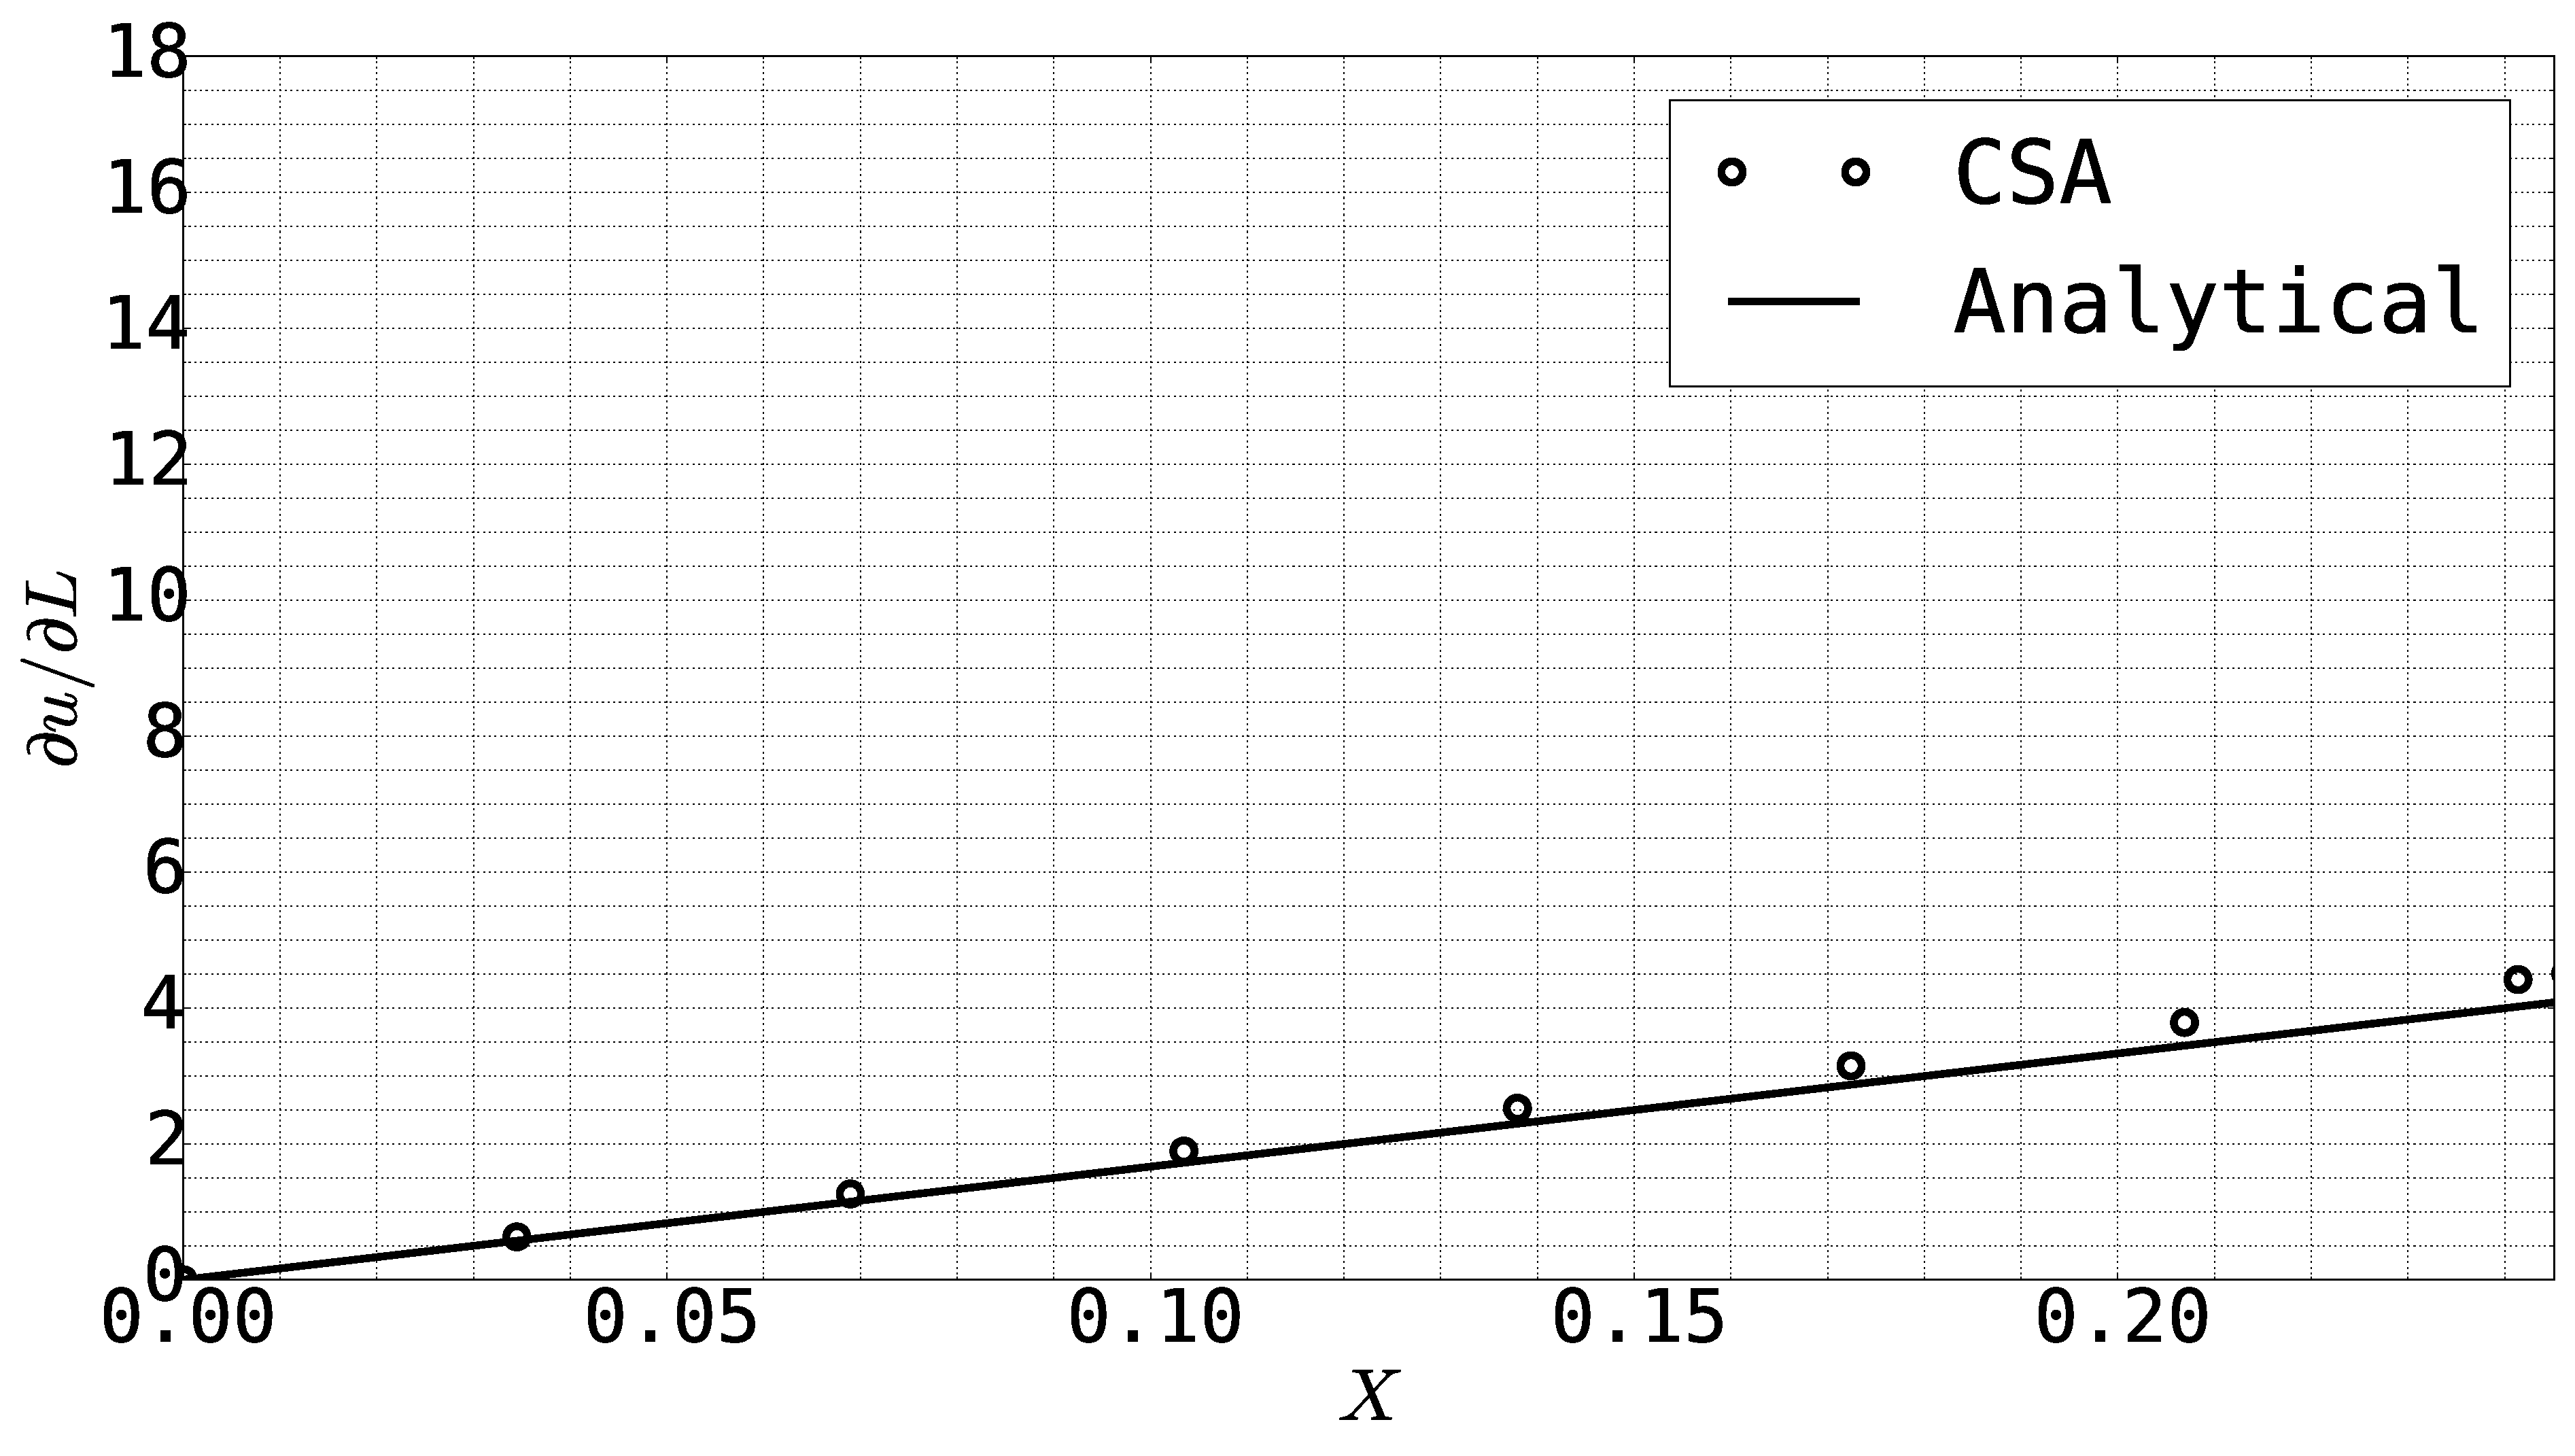
\includegraphics[width=7.0cm]{Chapter_4/figure/penalizationMethod_sensitivityProfile_reconstructed_xw02451.eps}
    }
    \quad
    \subfigure[$x_{wall} = 0.5742, n = 60$]
    {
    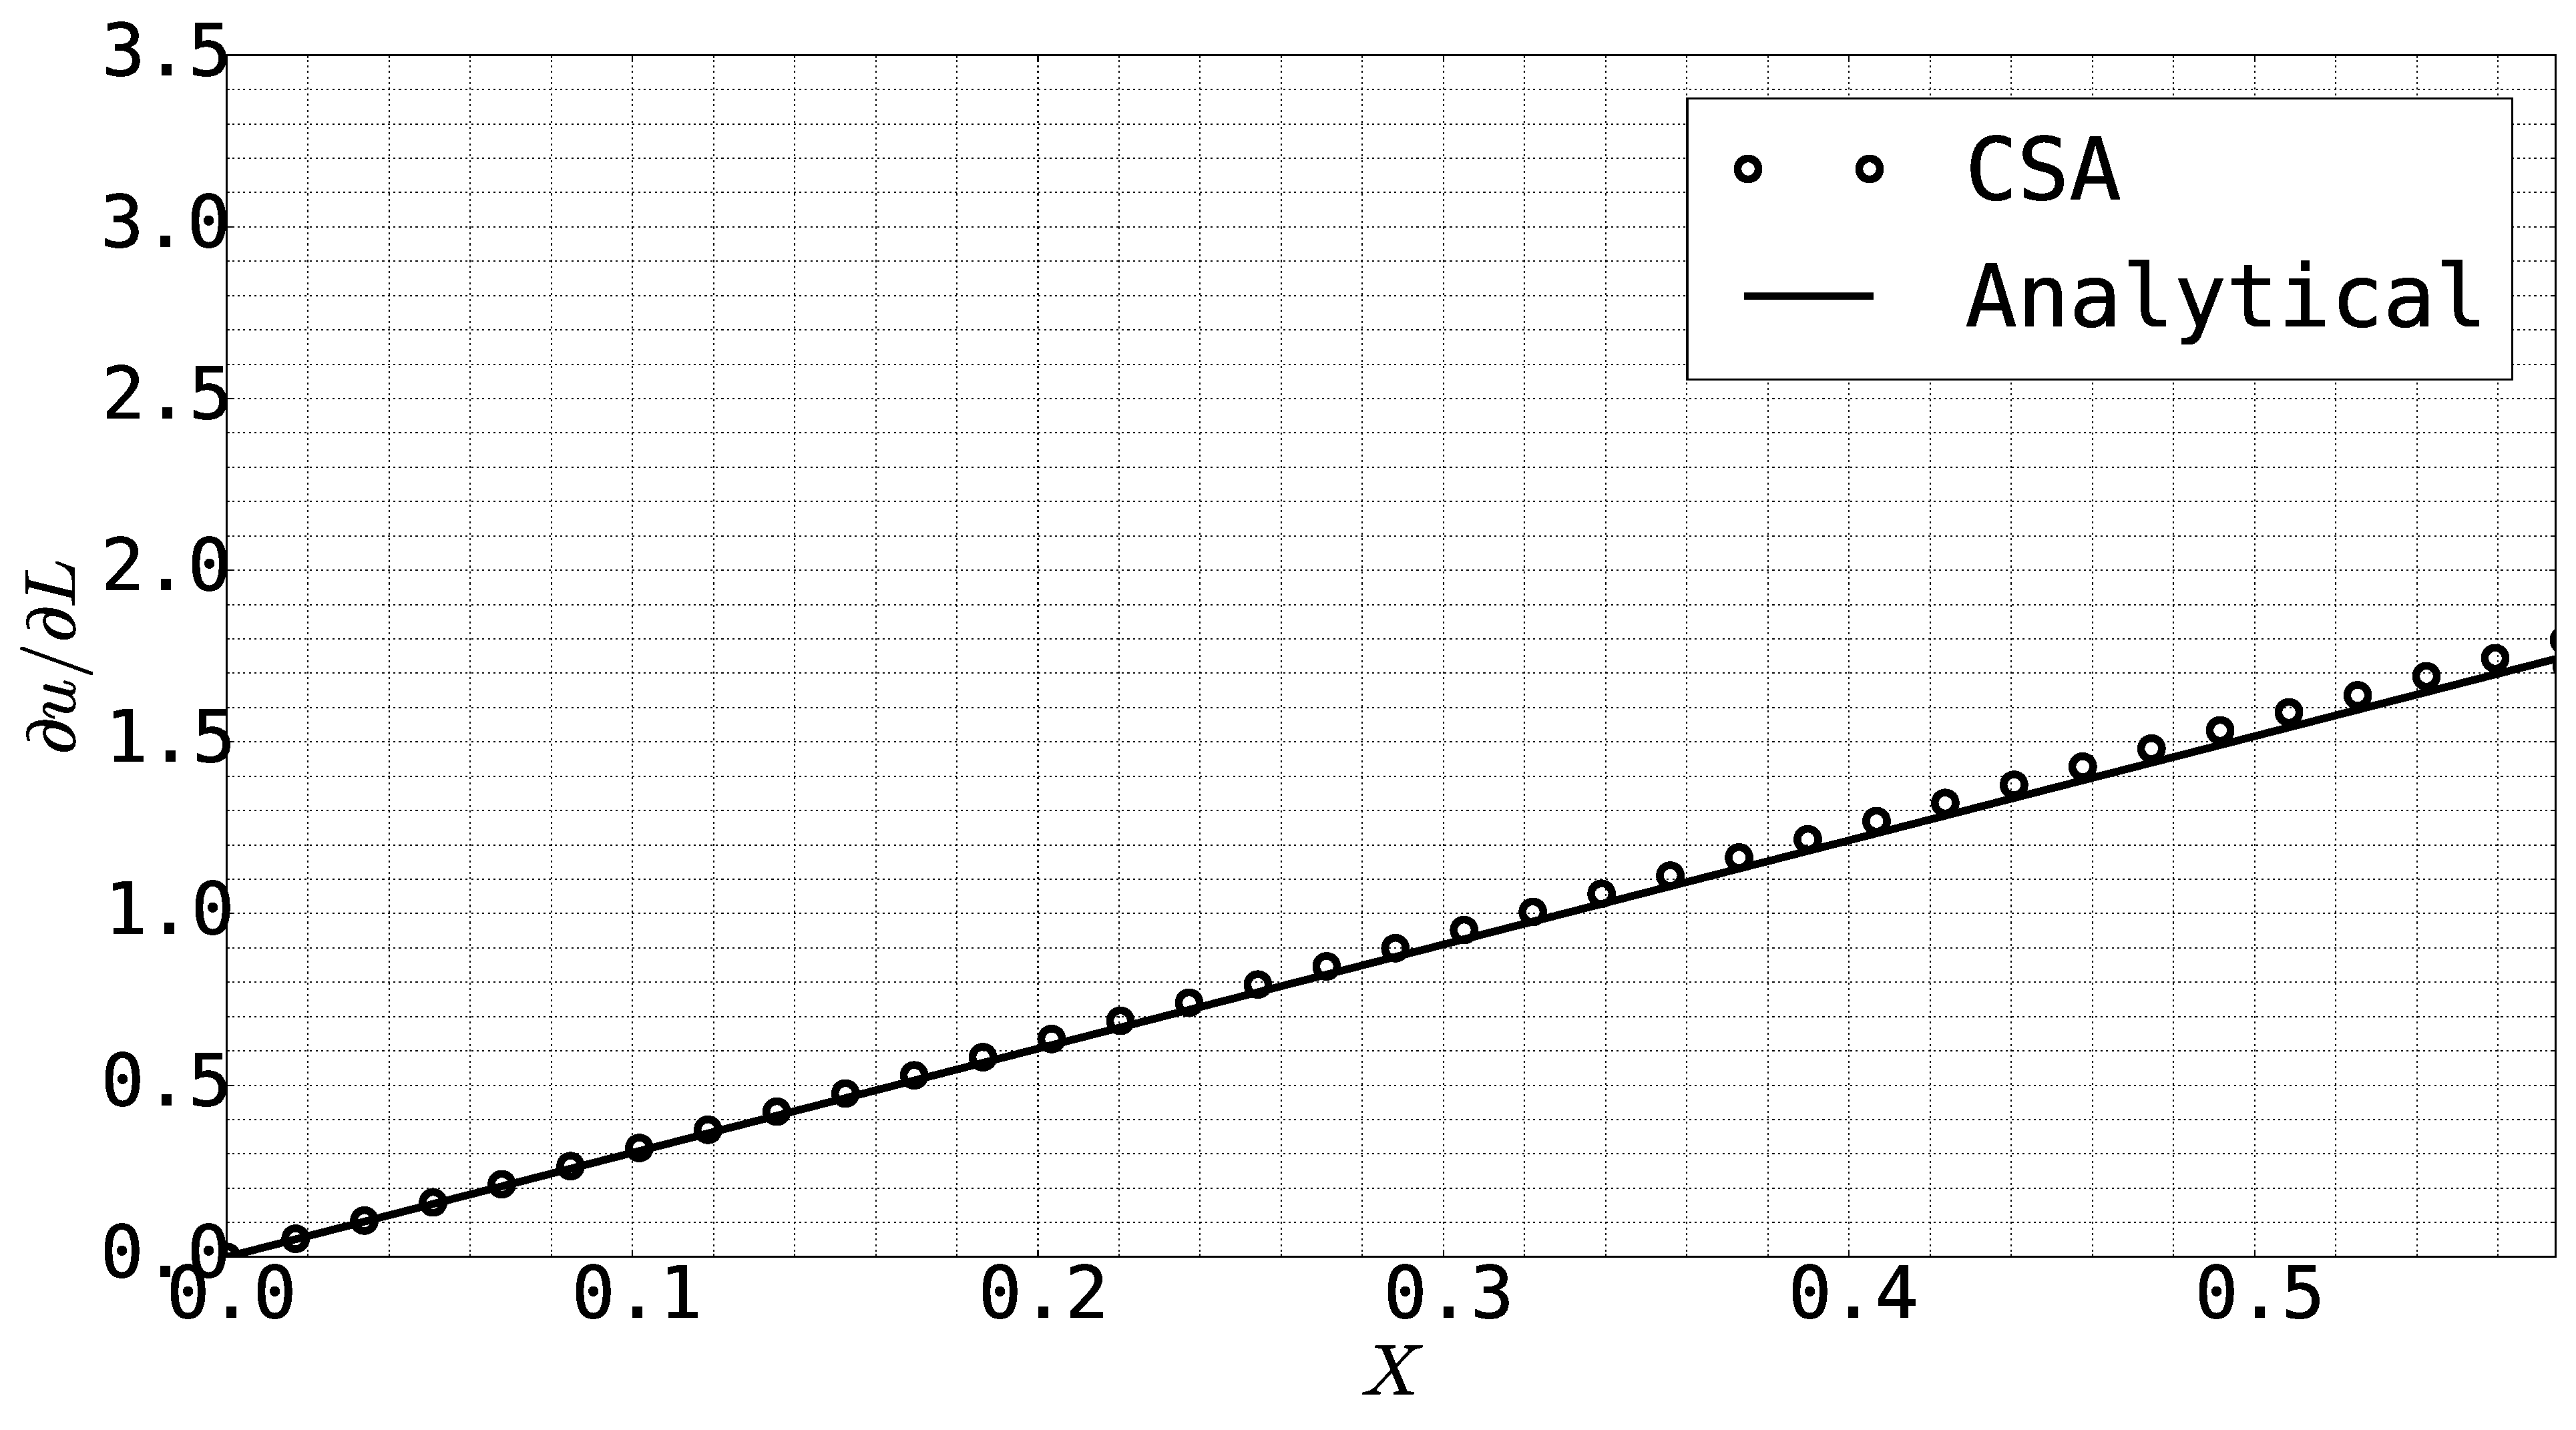
\includegraphics[width=7.0cm]{Chapter_4/figure/penalizationMethod_sensitivityProfile_reconstructed_xw05742.eps}
    }
    \caption{Reconstructed sensitivity by post-processing the results.}
    \label{fig:C4_sensitivityResultsReconstructed1Dproblem}
\end{figure}

This problem is also solved using the virtual boundary method.